\documentclass{article}

\usepackage{fullpage}

\usepackage[dvipsnames,svgnames,table]{xcolor}
\usepackage[colorlinks=true,linkcolor=RawSienna,citecolor=ForestGreen]{hyperref}

\usepackage[utf8]{inputenc}

\usepackage{amsthm}
\usepackage{thmtools}
\usepackage[normalem]{ulem}
\usepackage{mathtools,bm}
\usepackage[inline]{enumitem}
\usepackage{amsmath,amsfonts,amssymb,amsthm,hyperref,algorithm,eqparbox,array,ragged2e,stmaryrd,bbm}
\usepackage{xspace}
\usepackage{xcolor}
\usepackage{dsfont}
\usepackage{booktabs}
\usepackage[labelfont=bf]{caption}
\usepackage{wrapfig}
\usepackage{algpseudocode}
\usepackage{tocloft}
\usepackage[nottoc]{tocbibind} %Bibliography in ToC

\let\OLDthebibliography\thebibliography %% bibliography printout settings
\renewcommand\thebibliography[1]{
  \OLDthebibliography{#1}
  \setlength{\itemsep}{.4ex}
}


\usepackage[capitalise,nameinlink,noabbrev]{cleveref}

\usepackage{tikz}
\usetikzlibrary{positioning,fit}
\usepackage{tikz-3dplot}

%=== Theorem environments (registered with thmtools) ===
\declaretheorem[name=Theorem]{theorem}
\declaretheorem[name=Lemma]{lemma}
\declaretheorem[name=Proposition]{proposition}
\declaretheorem[name=Corollary]{corollary}

\declaretheorem[name=Conjecture]{conjecture}
\declaretheorem[name=Fact]{fact}
\declaretheorem[name=Assumption]{assumption}
\declaretheorem[name=Claim]{claim}

\theoremstyle{definition}
\declaretheorem[name=Definition]{definition}
\declaretheorem[name=Problem]{question}
\declaretheorem[name=Example]{example}

\theoremstyle{remark}
\declaretheorem[name=Remark]{remark}


\usepackage{thm-restate}

% Bold label in example environments
\makeatletter
\def\th@example{%
  \thm@notefont{}% same as heading font
  \normalfont % body font
}
\def\th@definition{%
  \thm@notefont{}% same as heading font
  \normalfont % body font
}
\makeatother


% =============================================

\DeclareMathOperator{\rk}{rk}
\DeclareMathOperator{\crk}{\overline{rk}}
\DeclareMathOperator{\sk}{sk}
\DeclareMathOperator{\csk}{\overline{sk}}
\DeclareMathOperator{\mar}{mar}
\DeclareMathOperator{\Rcc}{R}
\DeclareMathOperator{\Ucc}{U}
\DeclareMathOperator{\Dcc}{D}
\DeclareMathOperator{\Ccc}{C}
\DeclareMathOperator{\dist}{dist}



\DeclareMathOperator{\res}{res}
\DeclareMathOperator{\supp}{supp}

\renewcommand{\P}{\operatorname{P}}


\DeclareMathOperator{\EQ}{\textsc{Eq}}
\DeclareMathOperator{\HD}{\textsc{HD}}
\let\SS\undefined
\DeclareMathOperator{\SS}{\textsc{SS}}

\DeclareMathOperator{\xor}{\textsc{Xor}}
\DeclareMathOperator{\Rank}{\textsc{Rank}}
\DeclareMathOperator{\HW}{\textsc{HW}}
\DeclareMathOperator{\Parity}{\textsc{Parity}}
\DeclareMathOperator{\PRank}{\textsc{PRank}}

\DeclareMathOperator{\SK}{\textsc{SK}}

\newtheorem{step}{Step}


\crefname{example}{Example}{Examples}


\newcommand{\rankOne}{\Rank_{\leq 1}}

\title{\vspace{-3cm}Rank-One\vspace{-1cm}}

% \setlength{\parindent}{0pt}

\newcommand{\valentin}[1]{{\color{red}\textbf{VI:} #1 }}
\newcommand{\mika}[1]{{\color{Cerulean}\textbf{Mika:} #1 }}
\newcommand{\kaave}[1]{{\color{blue}\textbf{Kaave:} #1 }}
\newcommand{\anastasia}[1]{{\color{DarkOrchid}\textbf{Anastasia:} #1 }}

\usepackage[most]{tcolorbox}
\newtcbox{\dominobox}{
  on line,
  boxrule=0.5pt,
  arc=3pt,
  left=3pt,right=3pt,top=0pt,bottom=0pt,
  boxsep=0pt
}

\newcommand{\domino}[2]{%
  \,\dominobox{$\begin{matrix} #1 \\ #2 \end{matrix}$}\,%
}

%STANDARD COMMANDS
\newcommand{\N}{\mathbb{N}}
\newcommand{\Z}{\mathbb{Z}}
\newcommand{\R}{\mathbb{R}}
\newcommand{\C}{\mathbb{C}}
\newcommand{\Q}{\mathbb{Q}}
\newcommand{\T}{\mathbb{T}}
\newcommand{\One}{\mathds{1}}
\newcommand{\cP}{\mathcal{P}}
\newcommand{\cL}{\mathcal{L}}
\newcommand{\cI}{\mathcal{I}}
\newcommand{\cD}{\mathcal{D}}
\newcommand{\cX}{\mathcal{X}}
\newcommand{\cY}{\mathcal{Y}}
\newcommand{\cZ}{\mathcal{Z}}


%RENEWED COMMANDS
\renewcommand{\epsilon}{\varepsilon}
\renewcommand{\leq}{\leqslant}
\renewcommand{\geq}{\geqslant}
\renewcommand{\setminus}{\backslash}
\renewcommand{\Re}{{\rm Re}}
\renewcommand{\Im}{{\rm Im}}
\renewcommand{\subset}{\subseteq}
\renewcommand{\supset}{\supseteq}

\usetikzlibrary{
    babel,
    arrows,
	calc,
	patterns,
	intersections,
    backgrounds,
    trees,
    mindmap,
    fadings,
	decorations.pathreplacing,
	decorations.pathmorphing,
	decorations.text,
	decorations.markings,
    scopes,
	shapes,
	positioning,
    arrows.meta,
    math,
    shapes.geometric,
    calligraphy
}


% COLOURED BOXES


%\definecolor{resultcolor}{HTML}{FFE1D9}
\definecolor{resultcolor}{HTML}{EED7FC}
\definecolor{definitioncolor}{HTML}{FCDFBE}
%\definecolor{definitioncolor}{HTML}{EFF9BD}
%\definecolor{definitioncolor}{HTML}{FFE4B8}
\definecolor{questioncolor}{HTML}{DDE8EB}

\newenvironment{boxtheorem}{\begin{theorem}}{\end{theorem}}
\tcolorboxenvironment{boxtheorem}{colback=resultcolor, colframe=white, colbacktitle=resultcolor, coltitle=resultcolor}

\newenvironment{boxlemma}{\begin{lemma}}{\end{lemma}}
\tcolorboxenvironment{boxlemma}{colback=resultcolor, colframe=white, colbacktitle=resultcolor, coltitle=resultcolor}

\newenvironment{boxproposition}{\begin{proposition}}{\end{proposition}}
\tcolorboxenvironment{boxproposition}{colback=resultcolor, colframe=white, colbacktitle=resultcolor, coltitle=resultcolor}

\newenvironment{boxcorollary}{\begin{corollary}}{\end{corollary}}
\tcolorboxenvironment{boxcorollary}{colback=resultcolor, colframe=white, colbacktitle=resultcolor, coltitle=resultcolor}

\newenvironment{boxdefinition}{\begin{definition}}{\end{definition}}
\tcolorboxenvironment{boxdefinition}{colback=definitioncolor, colframe=white, colbacktitle=definitioncolor, coltitle=definitioncolor}

\newenvironment{boxquestion}{\begin{question}}{\end{question}}
\tcolorboxenvironment{boxquestion}{colback=questioncolor, colframe=white,
    colbacktitle=questioncolor, coltitle=questioncolor}


 


\begin{document}
\title{\mbox{}\\[0em]
\huge Algebraic Complexity Approach to Sign-Rank}

\author{
\mbox{}\\[-0.5em]
\setlength{\tabcolsep}{10pt}
\begin{tabular}{cccc}
    Mika G\"o\"os&
    Kaave Hosseini&
    Valentin Imbach&
    Anastasia Sofronova\\[-1mm]
    \small\slshape EPFL &
    \small\slshape University of Rochester &
    \small\slshape EPFL &
    \small\slshape EPFL
\end{tabular}}

\date{
\mbox{}\\[0em]
\today}

\maketitle

\begin{abstract}
\noindent
An outstanding open problem asks if there exists a boolean matrix with unbounded sign-rank, but bounded randomised communication complexity. We make progress towards this question by proving lower bounds against \emph{real linear sketches} (a model weaker than sign-rank): Alice and Bob send few linear measurements to a referee, who makes a decision based on the evaluation of a low-degree polynomial. Our proof uses the \emph{Combinatorial Nullstellensatz} and the \emph{rank method} from algebraic circuit complexity. 
 
\end{abstract}


\vspace{3em}
% \setlength{\cftbeforesecskip}{4pt}
% \renewcommand\cftsecfont{\mdseries}
\renewcommand{\cftsecpagefont}{\normalfont}
% \renewcommand{\cftsecleader}{\cftdotfill{\cftdotsep}}
\setcounter{tocdepth}{2}
\tableofcontents

\thispagestyle{empty}
\setcounter{page}{0}
\newpage


\section{Introduction}

The \emph{sign-rank} $\rk_\pm(M)$ of a boolean matrix $M\in\{0,1\}^{N\times N}$ is the least rank of a real matrix $S\in\R^{N\times N}$ such that~$\operatorname{sgn}(S_{ij}) = (-1)^{M_{ij}}$ for all~$i,j$. This notion was introduced by Paturi and Simon~\cite{PS86} and it has since been extensively studied in communication complexity and learning theory (see~\cref{sec:related-work} for references).
It corresponds to one of the most powerful models of communication, unbounded-error protocols. In fact, it is so powerful that several non-trivial matrices can have \emph{constant} sign-rank, independent of matrix size $N$:
\begin{itemize}[label=$-$,itemsep=0em]
    \item The \textsc{Equality} (or \emph{identity}) matrix ($ij$-th entry is 1 iff $i=j$) has sign-rank $3$.
    
    \item The \textsc{Greater-Than} matrix ($ij$-th entry is 1 iff $j\geq i$) has sign-rank $2$.
    
    \item The \textsc{$k$-Hamming Distance} ($k$-HD) matrices (rows/columns  indexed by binary strings; entry is $1$ iff Hamming distance between the strings equals $k$) have sign-rank $2^{O(k)}$~\cite{GHIS25}.
\end{itemize}
The final example, in particular, is surprising: before the constant upper bound was discovered, several papers~\cite{HHPTZ22,HHM23} had put forth the conjecture that $k$-HD should require super-constant sign-rank. 


\paragraph{Our problem.}
Despite decades of study, several fundamental problems about sign-rank remain poorly understood. In this paper, we address the following outstanding problem, which compares sign-rank with (public-coin) randomised communication complexity ($\Rcc$). The problem was first asked by Linial, Mendelson, Schechtman, and Shraibman~\cite{LMSS07} (although our formulation is from~\cite{HHPTZ22}). It asks ``merely'' to prove a super-constant sign-rank lower bound for a specific structured matrix. Nevertheless, the example of~$k$-HD demonstrates how tricky matrices of constant sign-rank can be.

\begin{boxquestion} \label{prob1}
Exhibit a matrix $M$ with $\Rcc(M)\leq O(1)$ but $\rk_\pm(M)\geq\omega(1)$.
\end{boxquestion}

This problem has several equivalent interpretations in communication complexity and learning theory, arising out of the many ways in which the class of matrices with $\Rcc(M)\leq O(1)$ can be characterised (constant discrepancy, point--halfspace arrangements with constant margin, PAC learnable under pure differential privacy); see \cref{sec:related-work} for these connections.

What makes \cref{prob1} particularly interesting is that most existing techniques yield lower bounds not only on $\rk_\pm(M)$ but also on $\Rcc(M)$. Indeed, Hatami, Hatami, Pires, Tao, and Zhao~\cite{HHPTZ22} discuss how existing methods (e.g.,~\cite{PS86,For02,APP+2005,AMY16}) all fail to resolve this problem. So far, the problem has been solved for \emph{partial} matrices by Hatami, Hosseini, and Meng~\cite{HHM23} who developed a novel lower-bound technique based on the Borsuk--Ulam theorem. For total matrices, \cref{prob1} has emerged as one of the foremost open problems in the study of \emph{constant-cost communication} (introduced in~\cite{HHH23,HWZ22} and surveyed in~\cite{HH24}) that treats two complexity measures as ``equivalent,'' if they can be bound as functions of one another, independent of $N$; see~\cref{fig:diagram}.

The $k$-HD matrices stood as promising candidates (proposed in~\cite{HHPTZ22,HHM23}) to witness the separation in \cref{prob1}, until the constant upper bound was discovered~\cite{GHIS25}. Currently, there exists only one known candidate matrix in the literature that is due to Sherstov and Storozhenko~\cite{SS24}.

\paragraph{Our contributions.} The goal of this paper is to make progress on \cref{prob1}:
\begin{itemize}
    \item We introduce a new communication model called \emph{real linear sketching} (see \cref{sec:sketch-def}). This model is weaker than sign-rank, but \emph{it captures the sign-rank upper bound for \textsc{$k$-HD} from}~\cite{GHIS25}.
    \item We resolve an analogue of \cref{prob1} by ruling out a class of constant-cost sketching protocols for the Sherstov--Storozhenko matrix (see~\cref{sec:main-result}). In particular, this means that \emph{the sign-rank upper bound technique from~{\upshape \cite{GHIS25}} does not extend to the Sherstov--Storozhenko matrix.} Our lower bound will crucially use the \emph{Combinatorial Nullstellensatz} and the central \emph{rank method} from algebraic circuit complexity.
\end{itemize}


\subsection{Our model: Real linear sketches} \label{sec:sketch-def}

\begin{figure}[t]
    \centering
    
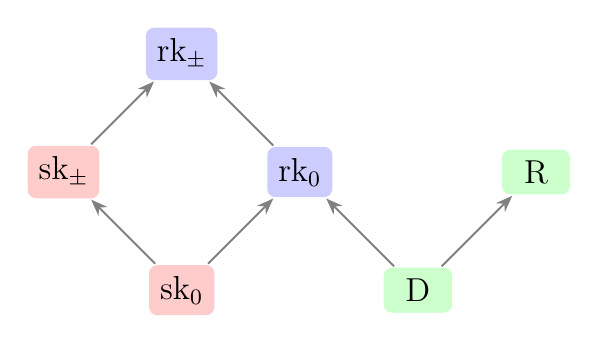
\begin{tikzpicture}[scale=1.5]
\tikzset{inner sep=0,outer sep=0.5}

% Set bounding box
%\node (a) at (-7.1,0) {\mbox{}};
%\node (b) at (7.1,0) {\mbox{}};

\tikzstyle{a}=[inner sep=4pt,fill=blue!20,rounded corners=3pt]
\tikzstyle{b}=[a, fill=red!20]

\begin{scope}[yscale=1]
\large
\node[a, fill = green!20] (D) at (0,0) {$\ \Dcc\ $};
\node[a] (rk0) at (-1,1) {$\rk_0$};
\node[a] (rkpm) at (-2,2) {$\rk_\pm$};
\node[a, fill = green!20] (R) at (1,1) {$\ \Rcc\ $};
\node[b] (sk0) at (-2,0) {$\sk_0$};
\node[b] (skpm) at (-3,1) {$\sk_\pm$};
\end{scope}


\path[-{Stealth[length=6pt]},line width=0.7pt,gray]
(D) edge (R)
(D) edge (rk0)
(rk0) edge (rkpm)
(sk0) edge (rk0)
(sk0) edge (skpm)
(skpm) edge (rkpm);


% \small
% \hypersetup{hidelinks}
% \tikzset{new/.style={-{Stealth[length=6pt]},dashed,line width=1pt,YellowOrange}}
% \draw[new,bend right=7]
% (Res) edge
% node[midway,below,inner sep=4pt,sloped] {\cref{thm:res-sa}}
% (uSA);
% \draw[new,bend right=20]
% (RevRes) edge
% node[pos=0.17,below,sloped,inner sep=3pt] {\cref{thm:revres-ns}}
% (FNS);

\end{tikzpicture}
        \caption{Relationships between complexity measures. An arrow $\Ccc_1 \longrightarrow\Ccc_2$ means that there is some function $\alpha\colon\N\to\N$ such that $\Ccc_2(M)\leq \alpha(\Ccc_1(M))$ for all matrices $M$. For example, the standard matrix rank ($\rk$) is equivalent to deterministic communication complexity ($\Dcc$) since $\log\rk(M)\leq\Dcc(M)\leq 2^{\rk(M)}$. In this paper, we introduce the sign-sketch ($\sk_\pm$) and support-sketch ($\sk_0$) complexities, which are naturally related to sign-rank ($\rk_\pm$) and support-rank ($\rk_0$). \cref{prob1} asks to show there is no arrow $\Rcc\longrightarrow\rk_\pm$.}
    \label{fig:diagram}
\end{figure}

From now on, we restrict our attention to $2^n$-by-$2^n$ boolean matrices corresponding to two-party functions of the form~$f\colon\{0,1\}^n\times\{0,1\}^n\to\{0,1\}$. In the following definition, the way a two-party function $f$ has chosen to represent its inputs (i.e., rows/columns) as $n$-bit strings is important: relabelling the inputs might change the sketching complexity of the function (which is not true for usual communication protocols).
\begin{boxdefinition}[Sketch protocols]
In a \emph{sketch protocol}, Alice receives input $x\in\{0,1\}^n$ and Bob receives input $y\in\{0,1\}^n$. The players each send $k$ linear measurements $Ax \in\R^k$ and $By\in\R^k$ (where~$A,B\colon\R^n \to \R^k$ are linear maps) to a third-party referee, who then makes a decision based on evaluating a fixed, degree-$d$, real polynomial $P\colon \R^{2k}\to\R$ on the $2k$ measurements $(Ax,By)$. We consider two possible acceptance criteria:
\begin{itemize}[label=$-$,noitemsep]
    \item \emph{Sign-sketch:} Referee accepts iff $P(Ax,By)> 0$.
    \item \emph{Support-sketch:} Referee accepts iff $P(Ax,By)\neq 0$.
\end{itemize}
The \emph{cost} of such a protocol is $k+d$. For a  function $f\colon\{0,1\}^n\times\{0,1\}^n\to\{0,1\}$, we define its \emph{sign-sketch complexity} $\sk_\pm(f)$ as the least cost of a sign-sketch protocol that computes $f$ correctly. The \emph{support-sketch complexity} $\sk_0(f)$ is defined similarly.
\end{boxdefinition}

\Cref{fig:diagram} shows how these new sketch complexities are related to previously studied  measures. It is easy to see that $\sk_\pm(f)\leq 2\sk_0(f)$, since we can simply square the polynomial $P$. 
Moreover, it is not hard to see that sign-sketches imply upper bounds on sign-rank (see~\cref{sec:prelim} for the proof). Analogously, support-sketches imply upper bounds on \emph{support-rank} $\rk_0(M)$, defined as the least rank of an $S\in\R^{N\times N}$ such that $M_{ij}=0$ iff $S_{ij}=0$, that is, $M$ and $S$ have the same support. Studying support-rank has proven particularly useful in past work, as it enjoys closure properties ($\land$ and $\lor$) incomparable to those for sign-rank ($\neg$ and $\oplus$).

To better grasp our new model, consider the following examples.

\begin{enumerate}[label=(E\arabic*),leftmargin=2.5em]
\item \label{ex:1}
The \emph{negation} of \textsc{Equality} ($\EQ$) admits a constant-cost support-sketch, that is, $\sk_0(\neg\EQ)\leq 2$. Each player just sends a single measurement, $Ax\coloneqq \sum_{i=1}^n2^i x_i$, and~$B\coloneqq A$. The referee then tests whether~$Ax\neq By$ via the $2$-variate degree-$1$ polynomial $P(a,b)\coloneqq a-b$. By contrast, we claim that~$\EQ$ itself has unbounded support-sketch complexity, $\sk_0(\EQ)\geq\omega(1)$. This follows from the stronger fact that its support-rank is unbounded; in fact, $\rk_0(\EQ)=2^n$.

\item \label{ex:2}
Our most important example is \textsc{$k$-Hamming Distance}. It is our chief motivation for the sketching model: the constant sign-rank upper bound from~\cite{GHIS25} can, in fact, be witnessed by a support-sketch.
In particular, the technique of the paper yields $\sk_0(\HD_{\geq k})\leq O(k^2)$ where $\HD_{\geq k}(x,y)\coloneqq 1$ iff the Hamming distance between $x,y\in\{0,1\}^n$ is at least $k$.

\item
Every function admits a support-sketch with $k=1$. Indeed, the players  choose $A$ and $B$ to be injective on their input domain $\{0,1\}^n$ (e.g., as in~\ref{ex:1}). The referee can then use interpolation to design a polynomial of huge degree (exponential in $n$) that vanishes precisely on $\{(Ax,By) : f(x,y)=0\}$.

\item \label{ex:4}
The \emph{parity} function has $\sk_\pm(\xor_{2n})\geq 2n$. This is because a degree-$d$ sign-sketch (regardless of~$k$) implies a degree-$d$ \emph{sign representation} (aka polynomial threshold representation) for $f(x,y)$, that is, a polynomial~$Q$ such that $\operatorname{sgn}(Q(x,y))=(-1)^{f(x,y)}$. It is a classic fact going back to Minsky and Papert~\cite{MP69} that the parity function requires full \emph{sign-degree} ($\deg_\pm$), namely $\deg_\pm(\xor_{2n})=2n$.
\end{enumerate}
The examples \ref{ex:1} and \ref{ex:4} demonstrate that our sketching models are incomparable to deterministic communication complexity, that is, there are no arrows $\sk_0\longrightarrow\Dcc$ and $\Dcc\longrightarrow\sk_\pm$  in \cref{fig:diagram}. While example~\ref{ex:4} identifies sign-degree as a lower bound on sketching complexity, $\sk_\pm(f)\geq\deg_\pm(f)$, our goal is to obtain sketching lower bounds even for functions of constant sign-degree, $\deg_\pm(f)\leq O(1)$. This includes, in particular, the Sherstov--Storozhenko function to be introduced next.


\subsection{Main results} \label{sec:main-result}

The Sherstov--Storozhenko~\cite{SS24} function is defined as follows. For input length $n=m^2$ we interpret the inputs $\smash{x,y\in\{0,1\}^n}$ as~$m$-by-$m$ boolean matrices, denote by $x\oplus y$ their modulo-2 sum, and set
\[
\SS(x,y)\coloneqq
\begin{cases}
1 &\text{if}\enspace \rk_{\mathbb{F}_2}(x\oplus y)>1, \\
0 &\text{else}.
\end{cases}
\]
In other words, $\SS(x,y)=0$ iff the 1-entries of $x\oplus y$ form a combinatorial rectangle (set of rows~$\times$ set of columns). Note that if the inputs to $\SS$ are restricted to be diagonal matrices, we recover the function~$\HD_{\geq 2}$. We conjecture that $\SS$ is strictly harder than $\HD_{\geq 2}$ for sign-rank, that is, $\rk_\pm(\SS)\geq \omega(1)$, and thus~$\SS$ would witness the separation in~\cref{prob1} (it is known~\cite{SS24,GHR25} that $\SS$ admits a constant-cost randomised protocol). However, at present, we are not able to show $\rk_0(\SS)\geq\omega(1)$ nor $\sk_\pm(\SS)\geq\omega(1)$. Instead, our main result shows a support-sketch lower bound. This implies, in particular, that the sign-rank upper bound technique for~$\HD_{\geq k}$ (example \ref{ex:2}) does not extend to $\SS$. 

\begin{boxtheorem} \label{thm:main}
    $\sk_0(\SS)\geq \Omega(n^{1/6})$.
\end{boxtheorem}

To prove \cref{thm:main}, we rely on several  tools (Combinatorial Nullstellensatz and the rank method) that have not been previously used in the study of sign-rank; see \cref{section:techniques} for a detailed proof overview.

\setlength{\columnsep}{1.8em}%
\begin{wrapfigure}{r}{0.28\textwidth}
\vspace{-1em}
\centering

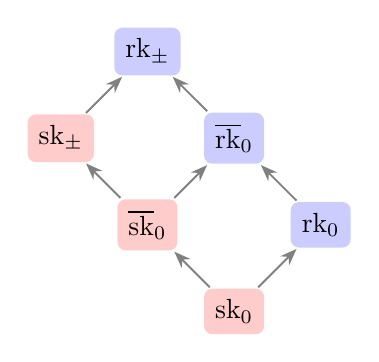
\begin{tikzpicture}[scale=1.1]
\tikzset{inner sep=0,outer sep=0.5}

% Set bounding box
%\node (a) at (-7.1,0) {\mbox{}};
%\node (b) at (7.1,0) {\mbox{}};

\tikzstyle{a}=[inner sep=4pt,fill=blue!20,rounded corners=3pt]
\tikzstyle{b}=[a, fill=red!20]

\begin{scope}[yscale=1]
\normalsize
\node[a] (rk0) at (-1,1) {$\rk_0$};
\node[a] (crk0) at (-2,2) {$\crk_0$};
\node[a] (rkpm) at (-3,3) {$\rk_\pm$};
\node[b] (sk0) at (-2,0) {$\sk_0$};
\node[b] (csk0) at (-3,1) {$\csk_0$};
\node[b] (skpm) at (-4,2) {$\sk_\pm$};
\end{scope}


\path[-{Stealth[length=6pt]},line width=0.7pt,gray]
(rk0) edge (crk0)
(crk0) edge (rkpm)
(sk0) edge (rk0)
(sk0) edge (csk0)
(csk0) edge (skpm)
(csk0) edge (crk0)
(skpm) edge (rkpm);



\end{tikzpicture}
    \caption{Boolean closures of support-rank/sketch.}
\vspace{-1em}
    \label{fig:boolean}
\end{wrapfigure}

\paragraph{Extension: Boolean closure.}
Support-rank lower bounds can sometimes feel brittle as the measure is not closed under complement. For instance, recall from \ref{ex:1} that $\rk_0(\neg\EQ)\leq O(1)$ while $\rk_0(\EQ)\geq\omega(1)$. In fact, one can show that $\rk_0(\neg\SS)\geq \omega(1)$ simply because $\neg\SS$ contains an unbounded-size $\EQ$ sub-matrix. To make sure that a support-rank/sketch result such as \cref{thm:main} is truly non-trivial---and hence provides some evidence that the sign-rank, too, is unbounded---it is desirable to extend the result to hold even against \emph{boolean closures}. Formally, an $n$-bit two-party function $f$ is a \emph{boolean combination} of some $n$-bit functions $f_1,\ldots,f_t$ if there exists some combining function $\Gamma\colon\{0,1\}^t\to\{0,1\}$ such that $f(x,y)=\Gamma(f_1(x,y),\ldots,f_t(x,y))$ for all~$x,y$. We define the \emph{boolean closure} $\crk_0(f)$  of support-rank as the minimum $\sum_i \rk_0(f_i)$ over all ways of expressing~$f$ as a boolean combination of $\{f_i\}$. The analogous closure for support-sketches, $\csk_0(f)$, is defined similarly. \cref{fig:boolean} illustrates how these measures relate to existing ones (see \cref{sec:prelim} for proofs). In particular, the boolean closures are still efficiently simulated by the corresponding sign measures.

We indeed show our \cref{thm:main} can be strengthened to hold against boolean closures. The paper~\cite{GHIS25} asked to prove lower bound against $\crk_0$ as a milestone towards~\cref{prob1}; the following theorem carries this out for the support-sketch model.

\begin{boxtheorem} \label{thm:main-ext}
    $\csk_0(\SS)\geq \omega(1)$.
\end{boxtheorem}



\subsection{Connection to algebraic circuit complexity}
 

A support-sketch can also be viewed as a constrained form of a nondeterministic polynomial representation. A nondeterministic polynomial for a boolean function $f$ is a polynomial $Q\in \mathbb{R}[x]$ such that
\[
    Q(x)\neq 0 \iff f(x)=1.
\] This notion was introduced by de Wolf in the context of quantum query complexity \cite{de2003nondeterministic}.
In our setting, the polynomial is required to have the more structured form $Q(x,y)=P(Ax,By)$, where $A$ and $B$ are rank-$k$ linear maps and $P$ has degree $d$. This can also be viewed as a form of depth-$3$ algebraic circuit complexity. 
If $Ax=(\ell_1(x),\ldots,\ell_k(x))$ and $By=(\ell_{k+1}(y),\ldots,\ell_{2k}(y))$, then 
\[
    P(\ell_1,\ldots,\ell_{2k}) = \sum_{|\alpha|\leq d} c_\alpha \prod_{i=1}^{2k}\ell_i^{\alpha_i},
\]
which gives a $\Sigma\Pi\Sigma$ circuit with product fan-in (middle layer) at most $d$ and top fan-in at most $\binom{2k+d}{d}.$ Moreover, all of its bottom linear forms lie in a space of
dimension at most $2k$. The dimension of span of bottom linear forms is known as \emph{rank} of the depth-3 circuit~\cite{saxena2011almost,shpilka2010arithmetic}, which is the minimum number of independent variables needed to express the circuit. 
In general, consider a real $\Sigma\Pi\Sigma$ circuit
\[
C(x,y)=
\sum_{i=1}^{t}
\prod_{j=1}^{d_i}
\ell_{i,j}(x,y), \quad
d\coloneqq\max_i d_i,
\]    
and let $r$ be its rank. In particular, $r\leq td$. It is easy to see that
\[d+r/2\leq \sk_0(C) \leq d+ r.\]
This gives a rephrasing of our main result (\Cref{thm:main}) as a real algebraic circuit lower bound.
\begin{boxtheorem}
[$\Sigma\Pi\Sigma$ lower bound]
Let $C(x,y)$ be a real $\Sigma\Pi\Sigma$ circuit with rank $r$ and maximum product fan-in $d$ such that, on boolean inputs $x,y\in\{0,1\}^n$,
\[C(x,y)\neq 0 \iff \SS(x,y)=1.\]
Then, $r+d\geq \Omega(n^{1/6})$.
\end{boxtheorem}
This lower bound is particularly curious in the context of  Polynomial Identity Testing (PIT); see surveys \cite{saxena2014progress,shpilka2010arithmetic}. Indeed, 
testing whether $\SS(x,y)=1$ is a simple PIT problem over $\mathbb{F}_2$.
Let $M=x\oplus y$ be viewed as an $m$-by-$m$ matrix over $\mathbb{F}_2$. Define a polynomial  $p_{M}\colon (\mathbb{F}_2^m)^4\to \mathbb{F}_2$ of degree four as
\[p_{M}(a_1,a_2,b_1,b_2) \coloneqq \det \begin{pmatrix}  
a_1^\top M b_1 & a_1^\top M b_2\\
a_2^\top M b_1 & a_2^\top M b_2 
\end{pmatrix} = (a_1^\top M b_1)( a_2^\top M b_2)+(a_1^\top M b_2)(a_2^\top M b_1).\]
It is easy to see that
\[p_{M} \equiv 0 \iff \rk_{\mathbb{F}_2}(M)\leq 1.\]
Thus, evaluating $p_{M}$ at random points $a_1,a_2,b_1,b_2\in\mathbb{F}_2^m$ gives a constant-query,
one-sided-error test for whether $\rk_{\mathbb{F}_2}(M)>1$. 
This is indeed the idea behind the constant-cost protocol for $\SS$~\cite{SS24,GHR25}.
Moreover, for every fixed choice of $a_1,a_2,b_1,b_2\in\mathbb{F}_2^m$, the polynomial 
\[C(x,y) \coloneqq p_{M}(a_1,a_2,b_1,b_2) = (a_1^\top (x\oplus y) b_1)( a_2^\top (x\oplus y) b_2)+(a_1^\top (x\oplus y) b_2)(a_2^\top (x\oplus y) b_1) \]
is a $\mathbb{F}_2$-$\Sigma\Pi\Sigma$ circuit with top fan-in and product fan-in 2, and rank at most 4. Moreover, it is easy to see that for a random choice of such $C$, if $\SS(x,y)=1$, then $C(x,y)=1$ with probability at least $2^{-4}$; and also if $\SS(x,y)=0$, then always $C(x,y)=0$. Taking constantly many samples  results in the following statement.
\begin{boxtheorem}
    There is a distribution over $\mathbb{F}_2$-$\Sigma\Pi\Sigma$ circuits $C$ of  constant rank and constant product fan-in  such that
    \[\Pr_{C}\left[C(x,y) = \SS(x,y)\right]\geq 2/3.\]
    Moreover, the error is one-sided; if $\SS(x,y)=0$ then $C(x,y)=0$.
\end{boxtheorem}

 
\subsection{Motivation and related work} \label{sec:related-work}

\paragraph{Unbounded-error communication.}
Paturi and Simon~\cite{PS86} showed that sign-rank characterises the communication complexity in the unbounded-error communication model ($\Ucc$), where randomness is private and the success probability is required to be strictly larger than $\frac{1}{2}$. Specifically, they showed that
\[
\Ucc(M) = \log{\rk_\pm(M)} \pm O(1).
\]
In particular, this means $\Ucc\longleftrightarrow \rk_\pm$ in the language of~\cref{fig:diagram}. Newman's theorem \cite{NEWMAN1991} states that public-coin randomness can be converted into private-coin randomness with just $O(\log{n})$ communication overhead. Thus, in particular, $\Ucc(M) \leq \Rcc(M) + O(\log{n})$. From this perspective, \Cref{prob1} asks whether one can get rid of the $O(\log n)$ dependence in this application of Newman's theorem. 

\paragraph{Margin and learning theory.}
There is also a geometric formulation via the \emph{margin complexity} $\mar(M)$ of a sign matrix $M\in\{\pm1\}^{N\times N}$. This is defined by
\[
\mar(M) \coloneqq \sup \min_{i,j} |\langle u_i,v_j\rangle|,
\]
where the supremum ranges over all dimensions and all unit vectors $u_i,v_j$ satisfying $M_{ij}=\operatorname{sgn}\langle u_i,v_j\rangle$. Sign-rank asks for a realisation in low dimension, whereas margin asks for a realisation with a large separation from the defining hyperplanes, with no restriction on the dimension. Constant-cost randomised protocols give constant-margin representations and vice versa~\cite{LMSS07}; that is, we have ``$\Rcc\longleftrightarrow\mar$'' in the language of \cref{fig:diagram}. Thus \Cref{prob1} can be viewed as asking whether constant margin implies constant-dimensional sign representations. Margin is a fundamental parameter in learning theory that controls the sample complexity of the support vector machine algorithm. The paper~\cite{LMSS07} observed that one can use the Johnson--Lindenstrauss lemma (in place of Newman's theorem) to upper bound sign-rank using margin with logarithmic dependence on the size of the matrix. From this perspective, \cref{prob1} asks whether one can get rid of the size dependence in this application of Johnson--Lindenstrauss. Finally, yet another characterisation of matrices with $\Rcc(M)\leq O(1)$ is that they correspond to PAC-learnability under pure differential privacy~\cite{FX14, BNS19}.  

We also mention that, very recently, several new frameworks and invariants for lower bounding sign-rank have been developed from a topological and learning theoretic perspective. Among them are lower bounding sign-rank by list replicability~\cite{chornomaz2025spherical,BHHLT26a, BHHLT26b}, or by $\Z_2$-index of certain simplicial complexes \cite{FHV26, BHHLT26b}, and approximate sign-rank lower bounds via a strengthening of Forster's method~\cite{BHKR26}.

\paragraph{Converse problem.}
The problem opposite of \cref{prob1} asks to construct matrices with small sign-rank but large randomised complexity. This direction was initiated by~\cite{babai1986complexity} and since then it has been studied exhaustively~\cite{buhrman2007computation, sherstov2008halfspace, sherstov2011pattern, Sherstov2013, Thaler2016, sherstov2021hardest,HHL20,ACHS24}. One culmination of this line of work~\cite{HHL20,ACHS24} exhibits a matrix of sign-rank $3$ but randomised complexity $\Omega(n)$.




\subsection{Open problems}

Our current method relies heavily on applying Combinatorial Nullstellensatz to the explicit polynomial $P$ in a support-sketch. Finding a support-rank analogue of this step is open, as is finding any technique to replace Nullstellensatz that can reason about the signs of a polynomial. This yields the following two incomparable challenge problems that serve as milestones towards \cref{prob1}.
 
\begin{boxquestion}
    Show $\rk_0(\SS)\geq \omega(1)$.
\end{boxquestion}

\begin{boxquestion}
    Show $\sk_\pm(\SS)\geq \omega(1)$.  
\end{boxquestion}


Another direction is to search for other candidate functions besides the function $\SS$. It is widely conjectured~\cite{GKPW18,CLV19,HHH23,HH24,GHRS26,Balla2025} that $\Rcc(f)\leq O(1)$ implies that $f$ contains a monochromatic rectangle of density $\Omega(1)$. (This is indeed satisfied by $\SS$.) Such constant-density monochromatic rectangles are known to exist for functions with $\rk_\pm(f)\leq O(1)$~\cite{APP+2005}. Thus, if this conjecture turns out to be false, the counterexample function would then witness the separation in \cref{prob1}, too.
 

\subsection{Proof overview of \Cref{thm:main}} \label{section:techniques}
We develop a general lower bound technique for any \emph{$\xor$-function}.
    We say that a function $f\colon\{0,1\}^n\times \{0,1\}^n\to\{0,1\}$ is an \emph{$\xor$-function} if for some $g\colon\{0,1\}^n\to \{0,1\}$ we have $f = g\circ \xor$, namely,
    \[
        \forall\, x,y\in \{0,1\}^n\ \colon\quad
        f(x, y) = g(x \oplus y).
    \]
Note that $\SS =\Rank_{>1}\circ\xor$ where for $x\in \mathbb{F}_2^{m\times m}$, $n=m^2$,
\[
\Rank_{>1}(x)\coloneqq
\begin{cases}
1 &\text{if}\enspace \rk_{\mathbb{F}_2}(x)>1, \\
0 &\text{else}.
\end{cases}
\]

At a high level, our proof of \Cref{thm:main} is an iterative degree-reduction argument.
We start with the polynomial $P$ from a given support-sketch computing a function $f$. We then find a small subset of variables of~$P$ that intersects all its top-degree monomials. By restricting these variables we obtain a polynomial $P'$ of smaller degree, while at the same time we make sure, using a ``self-reducibility'' property of $f$, that the restricted function $f'$ still computes a copy of~$f$, but on slightly fewer variables. Iterating this process eventually reduces the polynomial (and hence the function) to a constant. Since it takes several steps to reduce $f$ to a constant, it follows that $P$ must have had high degree to start with. This iterative procedure has two main ingredients, using \emph{Combinatorial Nullstellensatz}~\cite{alonCombinatorialNullstellensatz1999} and the \emph{rank method}~\cite{Nisan91}.


\paragraph{Nullstellensatz and no spread monomials.}
Let $g\colon\{0,1\}^n\to\{0,1\}$ and suppose $g(x\oplus y)=0$ if and only if $P(Ax,By)=0$ where $P$ has degree $d$ and $A,B$ are linear maps to $\R^k$. Consider the change of variables $z_i^+ = x_i+y_i$ and $z_i^- = x_i-y_i$. Hence $Q(z)\coloneqq P(Cz) = P(Ax,By)$ where $z = (z^+,z^-)\in \R^{2n}$ and
\[
C = \frac{1}{2}\begin{pmatrix}
    A & A\\
    B & -B
\end{pmatrix}.
\]
If we fix the parity $x_i\oplus y_i$ (to either 0 or 1), exactly one of $z_i^+,z_i^-$ becomes fixed and the other ranges over two values; see~\cref{fig:fixings}. We use this property to find for a given 0-input $a\in g^{-1}(0)$ a large product grid of corresponding inputs $z$ where~$Q(z)$ vanishes. Our goal is to show that this is impossible if $k+d$ is small. 

More specifically, for $g = \Rank_{>1}$, recall that the 0-inputs are precisely matrices whose $1$-entries form a combinatorial rectangle. In this case the coordinates of $z^+$ and $z^-$ are indexed by $[m]\times [m]$. Suppose a top-degree monomial $M$ of $Q$ is ``spread out'' meaning that the matrix entries corresponding to its (plus or minus type) variables are lying in distinct rows and columns. Based on the (plus or minus) type of each variable of $M$ we can prescribe entries of $x\oplus y$ in a way that $x\oplus y$ has rank at most 1 and all variables of $M$ independently vary over two values. The Combinatorial Nullstellensatz (\Cref{thm:nullstellensatz}) guarantees that $Q$ is non-zero somewhere on this grid, contradicting that the entire grid consists of 0-inputs of $Q$. In summary, this part implies that $Q$ does not have such ``spread-out'' top-degree monomials.

In the more general case, we capture the notion of ``spread-out'' based on some dependency graph defined for the function $g$ of interest. The corresponding statement is given in  \Cref{lem:xor-null}.

\paragraph{Rank method and no spread implies hitting sets.}
The second ingredient is to show that an absence of top-degree spread-out monomials of $Q$ forces global structure: all top-degree monomials of $Q$ can be hit by a few variables. In the case of $g = \Rank_{>1}$ the bound is $O(mkd)$.
To prove this, the key object of study here is a type of coefficient matrix $D_Q$ obtained from first derivatives of the top homogeneous part of $Q$. On the one hand, we show that the rank of $D_Q$ is upper-bounded by $k$, and, on the other hand, we show that if the top-degree monomials have no small hitting set, we can build a large triangular sub-matrix of $D_Q$ hence lower-bounding its rank. The final result is a second technical ingredient \Cref{lem:h-bound} which may be of independent interest. 

\paragraph{Iteration and putting the lemmas together.}
The first ingredient rules out spread-out top-degree monomials, and combined with the second, we get a small hitting set for all top degree monomials. We restrict all the variables in the hitting set which reduces the degree by one. Repeating for $d,d-1,\cdots,1$ gives a bound on the total number of variables. In the case of $g=\Rank_{>1}$ this is $O(mkd\times d) = O(mkd^2) = O(\sqrt{n}kd^2)$ which implies the bound of $\Omega(m^{1/3})$ on $k+d$, namely, the support-sketch complexity of the $\SS$ function.


\begin{figure}[t]
    \centering
    \def\arraystretch{1.2}
    \setlength\tabcolsep{.6em}
    \begin{tabular}{cc|c|cc}
    $x_i$ & $y_i$ & $x_i \oplus y_i$ & $z^+_i=x_i+y_i$ & $z^-_i=x_i-y_i$ \\
    \hline
    0 & 0 & 0 & 0 & \textbf{0} \\
    1 & 1 & 0 & 2 & \textbf{0} \\
    \hline
    0 & 1 & 1 & \textbf{1} & $-1$ \\
    1 & 0 & 1 & \textbf{1} & 1
    \end{tabular}
    \caption{Fixing $x_i\oplus y_i$ causes either $z^+_i$ or $z^-_i$ to become fixed while the other ranges over two values.}
    \label{fig:fixings}
\end{figure}




\section{Setup: Resilience and self-reducibility}
Our lower bound proof for $\SS=\Rank_{>1}\circ\xor$ works more generally for any function $f\circ \xor$ as long as~$f$ satisfies the following two properties, which we start formalising below.
\begin{itemize}[label=$-$,itemsep=0em]
    \item \emph{Resilience}, stating that certain partial inputs to $f$ can be completed to inputs that evaluate to $0$. This is used to construct the grid of inputs on which we apply the Combinatorial Nullstellensatz.
    \item \emph{Self-Reducibility}, stating that certain inputs of $f$ can be restricted in such a way that we recover $f$ on smaller inputs. We will use this to concentrate the complexity of $f$ in the top-degree of the polynomial.
\end{itemize}

\label{sec:proof-defs}

\subsection{Dependency graphs}
Both of the properties are defined relative to a \emph{dependency graph} $G$ on the input variables of~$f$, which we identify with $[n]$. Intuitively, an edge $i\sim_G j$ in this graph signifies that the two variables $x_i$ and $x_j$ are ``locally dependent'' on each other, in the context of evaluating $f$. We follow the convention that~$i \sim_G i$ for all $i\in [n]$, i.e.\ that each variable is dependent on itself. For $H \subseteq [n]$, define
\[
    N_G(H) = \{i\in [n]: i\sim_G j \text{ for some } j\in H \}.
\]
We sometimes drop the subscript $G$. Further, define $\Delta(G)$ as the maximal value of $|N_G(\{i\})|$ over all $i\in[n]$. We denote by $\varnothing$ the empty graph given by $i\sim_\varnothing j \iff i = j$. Note that $N_\varnothing(H) = H$ for all $H\subseteq [n]$ and $\Delta(\varnothing) = 1$. A set $S\subseteq [n]$ is \emph{independent} in $G$ if for any distinct $x,y\in S$ we have $x\not\sim y$.

When dealing with $\Rank_{>1}\circ\xor$, we will work relative to the dependency graph $G_{\Rank}$, given by
\[
    x_{ij} \sim_{G_{\Rank}} x_{i'j'} \iff i = i' \text{ or } j = j'.
\]
In other words, two variables are connected if and only if their corresponding entries in the matrix lie in the same row or column, see \Cref{fig:G}.
Intuitively, this is a good notion of ``local dependence'' when deciding if the $1$-entries form a combinatorial rectangle: The local obstruction of this fact consists of $3$ variables spanning just two rows and two columns, as illustrated in \Cref{fig:obstruction}. 

\begin{figure}[t]
    \centering
    \begin{minipage}{0.45\textwidth}
        \centering
        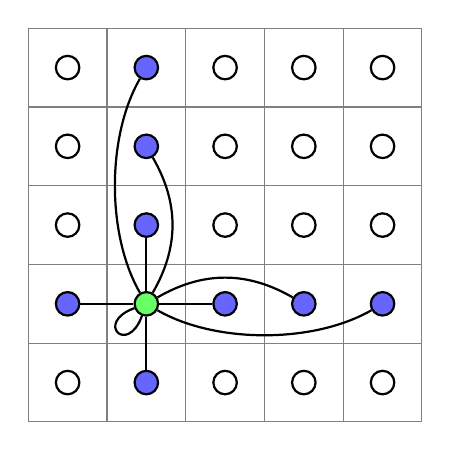
\begin{tikzpicture}

\draw[gray] (0,0) grid (5,5);

\node[circle, fill=green!60, inner sep=3pt] at (1.5,1.5) {};

\node[circle, fill=blue!60, inner sep=3pt] at (0.5,1.5) {};
\node[circle, fill=blue!60, inner sep=3pt] at (2.5,1.5) {};
\node[circle, fill=blue!60, inner sep=3pt] at (3.5,1.5) {};
\node[circle, fill=blue!60, inner sep=3pt] at (4.5,1.5) {};

\node[circle, fill=blue!60, inner sep=3pt] at (1.5,0.5) {};
\node[circle, fill=blue!60, inner sep=3pt] at (1.5,2.5) {};
\node[circle, fill=blue!60, inner sep=3pt] at (1.5,3.5) {};
\node[circle, fill=blue!60, inner sep=3pt] at (1.5,4.5) {};

\foreach \i in {1,...,5} {
    \foreach \j in {1,...,5} {
        \node[circle, draw=black, thick, inner sep=3pt] (v\i\j) at (\j-0.5,\i-0.5) {}; 
    }
}


\draw[thick] (v22) -- (v21);
\draw[thick] (v22) -- (v23);
\draw[thick] (v22) to[out=30, in=150] (v24);
\draw[thick] (v22) to[out=-30, in=-150,looseness=0.8] (v25);

\draw[thick] (v22) -- (v12);
\draw[thick] (v22) -- (v32);
\draw[thick] (v22) to[out=60, in=-60] (v42);
\draw[thick] (v22) to[out=120, in=-120,,looseness=0.8] (v52);

\draw[thick] (v22) to[out=-110,in=-160,looseness=10] (v22);

\end{tikzpicture}
        \vspace{-2em}
        \caption{The dependency graph $G_{\Rank}$ associated with the boolean function $\Rank_{> 1}$ on $\{0,1\}^{5\times 5}$. The neighbourhood of the green vertex $x_{4,1}$ is highlighted in blue.}
        \label{fig:G}
    \end{minipage}
    \hfill
    \begin{minipage}{0.45\textwidth}
        \centering
        
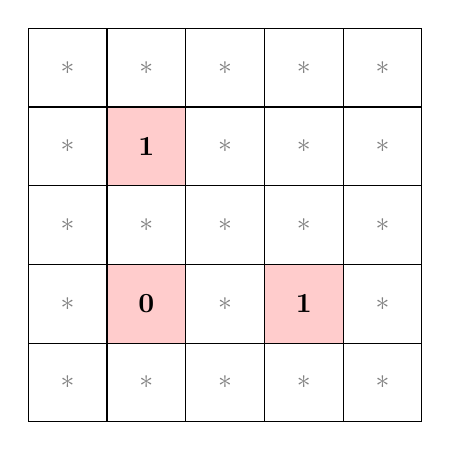
\begin{tikzpicture}

\fill[red!20] (1, -1) rectangle (2,-2);
\fill[red!20] (1, -3) rectangle (2,-4);
\fill[red!20] (3, -3) rectangle (4,-4);

% Matrix grid
\draw (0,0) grid (5,-5);

% Matrix entries
\node[text=gray] at (0.5,-0.5) {$*$};
\node[text=gray] at (1.5,-0.5) {$*$};
\node[text=gray] at (2.5,-0.5) {$*$};
\node[text=gray] at (3.5,-0.5) {$*$};
\node[text=gray] at (4.5,-0.5) {$*$};

\node[text=gray] at (0.5,-1.5) {$*$};
\node[font=\bfseries] at (1.5,-1.5) {1};
\node[text=gray] at (2.5,-1.5) {$*$};
\node[text=gray] at (3.5,-1.5) {$*$};
\node[text=gray] at (4.5,-1.5) {$*$};

\node[text=gray] at (0.5,-2.5) {$*$};
\node[text=gray] at (1.5,-2.5) {$*$};
\node[text=gray] at (2.5,-2.5) {$*$};
\node[text=gray] at (3.5,-2.5) {$*$};
\node[text=gray] at (4.5,-2.5) {$*$};

\node[text=gray] at (0.5,-3.5) {$*$};
\node[font=\bfseries] at (1.5,-3.5) {0};
\node[text=gray] at (2.5,-3.5) {$*$};
\node[font=\bfseries] at (3.5,-3.5) {1};
\node[text=gray] at (4.5,-3.5) {$*$};

\node[text=gray] at (0.5,-4.5) {$*$};
\node[text=gray] at (1.5,-4.5) {$*$};
\node[text=gray] at (2.5,-4.5) {$*$};
\node[text=gray] at (3.5,-4.5) {$*$};
\node[text=gray] at (4.5,-4.5) {$*$};

\end{tikzpicture}
        \vspace{-2em}
        \caption{The three red entries form a ``corner'' with $1$s at the tips and a $0$ at the joint. This is a local obstruction to the $1$-entries forming a combinatorial rectangle.}
        \label{fig:obstruction}
    \end{minipage}
\end{figure}

\subsection{Resilience}

Recall that for a boolean function $f\colon\{0,1\}^n\to\{0,1\}$ and some $I \subseteq [n]$, a \emph{restriction} of $f$ on $I$ is a function~$f'\colon \{0,1\}^{n-|I|}\to \{0,1\}$ obtained by fixing the variables indexed by $I$ to some boolean values.
\begin{boxdefinition}[Resilience]
    Let $f\colon\{0,1\}^n\to \{0,1\}$ and let $G$ be a graph on $[n]$. The \emph{resilience} of $f$ with respect to $G$, written $\res_G(f)$, is the largest integer $t$ with the following property:
    For every independent set $S$ in $G$ with $|S|\leq t$ and every restriction of $f$ on $S$, the resulting function is non-constant. If there is no largest such integer, we set $\res_G(f) = \infty$.
\end{boxdefinition}

\begin{example}\label{ex:resiliance}
    We have $\res_\varnothing(\HW_{\geq k}) = k-1$ (assuming $n > k$), where $\HW_{\geq k}$ is the function that accepts all $n$-bit strings of Hamming weight $\geq k$. Also, $\res_\varnothing(\Parity) = n-1$, where $\Parity$ is the function that accepts all $n$-bit strings with odd Hamming weight. Finally, $\res_{G_{\Rank}}(\Rank_{>1}) = \infty$, since no restriction on any independent set is constant, see \Cref{fig:resilience}.
\end{example}

\subsection{Self-reducibility}

\begin{boxdefinition}[Self-reducibility]
    Let $f=(f_n)$ be a family of functions and let $G=(G_n)$ be a corresponding family of dependency graphs on $[n]$, where $\Delta(G_n)$ is non-decreasing in $n$. We say $f$ is $G$-\emph{self-reducible} if for every set of variables indexed by $I\subseteq [n]$ with $|I|<n/\Delta(G_n)$, there is a restriction of $f_n$ on a superset of $N(I)$ which recovers some $f_{n'}$ with input size $n' \geq n - \Delta(G_n)|I|$.    
\end{boxdefinition}

\begin{example}\label{ex:self-reducibility}
    Both $\HW_{\geq k}$ and $\Parity$ are $\varnothing$-self-reducible, since after restricting some variables to zero, we recover the same function, just on a smaller domain.

    Moreover, $\Rank_{>1}$ is $G_{\Rank}$-self-reducible:
    Note that $\Delta(G_{\Rank}) = 2\sqrt{n}-1$ and let $I$ be a set of variables of $\Rank_{>1}$ with $|I| \leq \sqrt{n}$.
    When $\Rank_{>1}$ is restricted on $N_{G_{\Rank}}(I)$, the unrestricted inputs still contain a combinatorial square $R$ of side length at least $\sqrt{n}-|I|$. Restricting all entries outside of $R$ to $0$, we recover the function $\Rank_{>1}$ on input length $(\sqrt{n} - |I|)^2 \geq n - \Delta(G_{\Rank})\cdot |I|$. This is illustrated in \Cref{fig:self-reducibility}.
\end{example}

\begin{figure}[t]
    \centering
    \begin{minipage}{0.45\textwidth}
        \centering
        
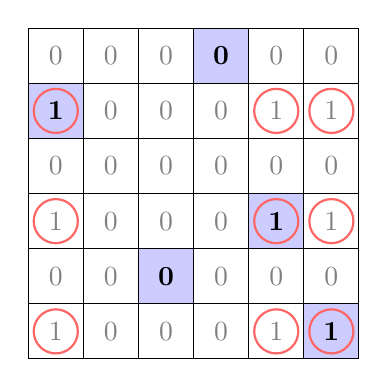
\begin{tikzpicture}[scale=0.7]

% Highlighted squares
\fill[blue!20] (0,-1) rectangle (1,-2);
\fill[blue!20] (2,-4) rectangle (3,-5);
\fill[blue!20] (3, 0) rectangle (4,-1);
\fill[blue!20] (4,-3) rectangle (5,-4);
\fill[blue!20] (5,-5) rectangle (6,-6);

\draw[red!60, thick] (0.5,-1.5) circle (0.4);
\draw[red!60, thick] (4.5,-1.5) circle (0.4);
\draw[red!60, thick] (5.5,-1.5) circle (0.4);

\draw[red!60, thick] (0.5,-3.5) circle (0.4);
\draw[red!60, thick] (4.5,-3.5) circle (0.4);
\draw[red!60, thick] (5.5,-3.5) circle (0.4);

\draw[red!60, thick] (0.5,-5.5) circle (0.4);
\draw[red!60, thick] (4.5,-5.5) circle (0.4);
\draw[red!60, thick] (5.5,-5.5) circle (0.4);

% Bold highlighted bits
\node[font=\bfseries] at (0.5,-1.5) {1};
\node[font=\bfseries] at (2.5,-4.5) {0};
\node[font=\bfseries] at (4.5,-3.5) {1};
\node[font=\bfseries] at (3.5,-0.5) {0};
\node[font=\bfseries] at (5.5,-5.5) {1};

% Matrix grid
\draw (0,0) grid (6,-6);

% Matrix entries
\node[text=gray] at (0.5,-0.5) {0};
\node[text=gray] at (1.5,-0.5) {0};
\node[text=gray] at (2.5,-0.5) {0};
\node[text=gray] at (4.5,-0.5) {0};
\node[text=gray] at (5.5,-0.5) {0};

\node[text=gray] at (1.5,-1.5) {0};
\node[text=gray] at (2.5,-1.5) {0};
\node[text=gray] at (3.5,-1.5) {0};
\node[text=gray] at (4.5,-1.5) {1};
\node[text=gray] at (5.5,-1.5) {1};

\node[text=gray] at (0.5,-2.5) {0};
\node[text=gray] at (1.5,-2.5) {0};
\node[text=gray] at (2.5,-2.5) {0};
\node[text=gray] at (3.5,-2.5) {0};
\node[text=gray] at (4.5,-2.5) {0};
\node[text=gray] at (5.5,-2.5) {0};

\node[text=gray] at (0.5,-3.5) {1};
\node[text=gray] at (1.5,-3.5) {0};
\node[text=gray] at (2.5,-3.5) {0};
\node[text=gray] at (3.5,-3.5) {0};
\node[text=gray] at (5.5,-3.5) {1};

\node[text=gray] at (0.5,-4.5) {0};
\node[text=gray] at (1.5,-4.5) {0};
\node[text=gray] at (3.5,-4.5) {0};
\node[text=gray] at (4.5,-4.5) {0};
\node[text=gray] at (5.5,-4.5) {0};

\node[text=gray] at (0.5,-5.5) {1};
\node[text=gray] at (1.5,-5.5) {0};
\node[text=gray] at (2.5,-5.5) {0};
\node[text=gray] at (3.5,-5.5) {0};
\node[text=gray] at (4.5,-5.5) {1};

\end{tikzpicture}
        \vspace{-2em}
        \caption{After fixing some entries on a $G_{\Rank}$-independent set (in blue), we can still choose to either create a $1$-rectangle (in red), or to avoid it. Thus, $\res_G(\Rank_{>1}) = \infty$.}
        \label{fig:resilience}
    \end{minipage}
    \hfill
    \begin{minipage}{0.45\textwidth}
        \centering
        
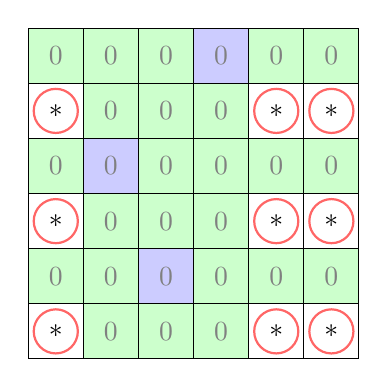
\begin{tikzpicture}[scale=0.7]

% Highlighted squares
\fill[green!20] (1,0) rectangle (4,-6);
\fill[green!20] (0,0) rectangle (6,-1);
\fill[green!20] (0,-2) rectangle (6,-3);
\fill[green!20] (0,-4) rectangle (6,-5);

\fill[blue!20] (1,-2) rectangle (2,-3);
\fill[blue!20] (2,-4) rectangle (3,-5);
\fill[blue!20] (3, 0) rectangle (4,-1);

\draw[red!60, thick] (0.5,-1.5) circle (0.4);
\draw[red!60, thick] (4.5,-1.5) circle (0.4);
\draw[red!60, thick] (5.5,-1.5) circle (0.4);

\draw[red!60, thick] (0.5,-3.5) circle (0.4);
\draw[red!60, thick] (4.5,-3.5) circle (0.4);
\draw[red!60, thick] (5.5,-3.5) circle (0.4);

\draw[red!60, thick] (0.5,-5.5) circle (0.4);
\draw[red!60, thick] (4.5,-5.5) circle (0.4);
\draw[red!60, thick] (5.5,-5.5) circle (0.4);

% Matrix grid
\draw (0,0) grid (6,-6);

% Matrix entries
\node[text=gray] at (0.5,-0.5) {0};
\node[text=gray] at (1.5,-0.5) {0};
\node[text=gray] at (2.5,-0.5) {0};
\node[text=gray] at (3.5,-0.5) {0};
\node[text=gray] at (4.5,-0.5) {0};
\node[text=gray] at (5.5,-0.5) {0};

\node at (0.5,-1.5) {$*$};
\node[text=gray] at (1.5,-1.5) {0};
\node[text=gray] at (2.5,-1.5) {0};
\node[text=gray] at (3.5,-1.5) {0};
\node at (4.5,-1.5) {$*$};
\node at (5.5,-1.5) {$*$};

\node[text=gray] at (0.5,-2.5) {0};
\node[text=gray] at (1.5,-2.5) {0};
\node[text=gray] at (2.5,-2.5) {0};
\node[text=gray] at (3.5,-2.5) {0};
\node[text=gray] at (4.5,-2.5) {0};
\node[text=gray] at (5.5,-2.5) {0};

\node at (0.5,-3.5) {$*$};
\node[text=gray] at (1.5,-3.5) {0};
\node[text=gray] at (2.5,-3.5) {0};
\node[text=gray] at (3.5,-3.5) {0};
\node at (4.5,-3.5) {$*$};
\node at (5.5,-3.5) {$*$};

\node[text=gray] at (0.5,-4.5) {0};
\node[text=gray] at (1.5,-4.5) {0};
\node[text=gray] at (2.5,-4.5) {0};
\node[text=gray] at (3.5,-4.5) {0};
\node[text=gray] at (4.5,-4.5) {0};
\node[text=gray] at (5.5,-4.5) {0};

\node at (0.5,-5.5) {$*$};
\node[text=gray] at (1.5,-5.5) {0};
\node[text=gray] at (2.5,-5.5) {0};
\node[text=gray] at (3.5,-5.5) {0};
\node at (4.5,-5.5) {$*$};
\node at (5.5,-5.5) {$*$};

\end{tikzpicture}
        \vspace{-2em}
        \caption{For any set of variables $I$ (in blue) of $\Rank_{>1}$, there is a restriction (to zero) on a superset of $N(I)$ (in green) which recovers $\Rank_{>1}$ (in red). Thus, $\Rank_{>1}$ is $G_{\Rank}$-self-reducible.}
        \label{fig:self-reducibility}
    \end{minipage}
\end{figure}

\section{Proof of main result (\Cref{thm:main})}
 The proof of \Cref{thm:main} immediately follows from the following more general lemma. 
  Indeed, we have seen that~$\Rank_{>1}$ is $G_{\Rank}$-self-reducible in \Cref{ex:self-reducibility}. We also know that $\res_{G_{\Rank}}(\Rank_{>1}) = \infty$ from \Cref{ex:resiliance} and $\Delta(G_{\Rank}) = 2\sqrt{n}-1$. Plugging these facts in the lemma below proves \Cref{thm:main}.


\begin{boxlemma}\label{lem:main-tec}
     Let $f=(f_n)$ be a $G_n$-self-reducible family. If $\res_{G_n}\!(f_n) \geq \Omega(n/\Delta(G_n))^{1/3}$, then
    \[
        \sk_0(f_n\circ\xor) \geq \Omega(n/\Delta(G_n))^{1/3}.
    \]
\end{boxlemma}

The proof of \Cref{lem:main-tec} follows from the next two \Cref{lem:xor-null,lem:h-bound}. We postpone their proofs to \Cref{subsection:xor-null-proof,sec:rank-method} respectively, since it requires the introduction of new concepts. To state the lemmas, we first need to define notions of \emph{independence} and \emph{hitting sets}. 
 \paragraph{Independent and hitting sets.}
For a monomial $M$ appearing in $P\in \mathbb{R}[x_1,x_2,\dots, x_n]$, write  $\supp(M)$ for the multiset of indices of the variables appearing in $M$. Given a graph $G$ on $[n]$, we call $M$ \emph{independent} in $G$ if $M$ is multilinear and $\supp(M)$ is an independent set in $G$.
Further, we denote by $G^{(2)}$ the graph on $[2n]$ given by
\[
    i \sim_{G^{(2)}} j \iff (i\ \operatorname{mod}\ n)\sim_G (j\ \operatorname{mod}\ n).
\]
Furthermore, let $\mathcal{M}$ be the family of all top-degree monomials of $P$.   A set $H\subset [n]$  is a \emph{$G$-hitting set} of $P$ if 
    \[
        \forall M\in \mathcal{M}: \quad \supp(M)\cap N(H)\neq \varnothing.
    \]
    We denote by $h_G(P)$ the size of the smallest $G$-hitting set in $P$.
\paragraph{The main technical lemmas.}
The next lemma is where we apply Combinatorial Nullstellensatz.
\begin{boxlemma}\label{lem:xor-null}
    Let $f\colon\{0,1\}^n\to \{0,1\}$ and let $G$ be a graph on $[n]$. 
    Let $P$ be a real, degree-$d$ polynomial over $2n$ variables such that
    \[
        \forall x,y\in \{0,1\}^n\colon\quad
        f(x \oplus y) = 0 \iff P(x+y,\ x-y) = 0.
    \]
    If $\res_G(f) \geq d$, then $P$ has no degree-$d$ monomial 
    which is independent in $G^{(2)}$.
\end{boxlemma}
% We postpone the proof of \Cref{lem:xor-null} to \Cref{subsection:xor-null-proof}.
 
The dual notions of independent set and hitting set are usually related as follows: Independent set size is a lower bound on hitting set size. The following lemma provides a converse to this paradigm in our setting.

\begin{boxlemma}\label{lem:h-bound}
    Let $P \in \mathbb{R}[x_1,\dots,x_k]$ and, $A:\R^n\to \R^k$ linear, and $G$ a graph on $[n]$.
    Let $Q(x) \coloneqq P(Ax)$ and suppose that $Q$ is non-zero and $d = \deg(Q)$. If $Q$ has no top-degree monomial which is independent in $G$, then $h_G(Q) \leq dk$.
\end{boxlemma}

\begin{proof}[Proof of \Cref{lem:main-tec}]
    Let $\Delta_n = \Delta(G_n)$. Suppose that $f_n\circ \xor$ has a support-sketch protocol with $k$ sketches and a degree-$d$ polynomial $P$. For a contradiction, assume that there is a constant $0 < c < 2^{-1/3}$ with
    \[
           k+d \leq c\left(\frac{n}{\Delta_n}\right)^{1/3} \leq\  \frac{\res_{G_n}(f_n)}{2}.
    \]
    We repeatedly apply the following reduction argument, which decreases both the input size $m$ and the degree $d_m$. We will ensure that $m \geq n/2$, where by monotonicity of $\Delta_m$ we have
    \begin{equation}\label{eq:assumption}
        \res_{G_m}(f_m)
        \geq
        2c\left(\frac{m}{\Delta_m}\right)^{1/3}
        \geq c\left(\frac{n}{\Delta_n}\right)^{1/3}\geq d.
    \end{equation}
    
    Given a sketch-protocol for $f_m\circ \xor$ with polynomial $P_m$ of degree $d_m$, we perform the change of variables $z^+ = x+y$ and $z^-=x-y$. Then, by \Cref{lem:xor-null,lem:h-bound}, we get a $G_m^{(2)}$-hitting set $H$ of size at most $2d_m k$. Let $I$ denote the set of variables of $f_m$ by collapsing $z^+_i$ with $z^-_i$ in $H$. Note that $|I| \leq |H| \leq 2d_m k$. By self-reducibility, we can restrict a superset of $N(I)$ to recover $f_{m'}$, where 
    \[
        m'\geq m-\Delta_m|I| \geq m - 2k\Delta_m d_m.
    \]
    Performing this restriction to both the $z^+$ and $z^-$ variables, we recover $f_{m'}\circ\xor$ and a new support-sketch protocol with polynomial $P_{m'}$ of degree $d_{m'}$. But since $H$ was a $G^{(2)}_m$-hitting set, we must have $d_{m'} < d_m$.
    Repeating this, we reach degree $0$ while the overall loss in input size is at most 
    \[
        2k\Delta_n\sum_{i=1}^d i\leq k\Delta_n d(d+1) \leq \Delta_n(k+d)^3 \leq c^3n \leq n/2,
    \]
    ensuring that \Cref{eq:assumption} holds at every step.
    Hence, we have arrived at a non-constant function $f_m$ with a degree-zero support-sketch protocol, which is a contradiction.
\end{proof}



\subsection{Combinatorial Nullstellensatz and proof of \Cref{lem:xor-null}}
\label{subsection:xor-null-proof}

Our goal in this subsection is to prove \Cref{lem:xor-null}. The key observation is that 0-inputs of an XOR-function naturally give rise to product grids in the variables $x+y$ and $x-y$. If a top-degree monomial of the sketching polynomial is sufficiently spread out, then one can choose such a grid on which the polynomial must vanish identically, while the Combinatorial Nullstellensatz guarantees that it is non-zero at some point of the grid. This contradiction rules out independent top-degree monomials.


\begin{boxtheorem}[Combinatorial Nullstellensatz~\cite{alonCombinatorialNullstellensatz1999}]
\label{thm:nullstellensatz}
Let $P \in \R[x_1, \ldots, x_n]$ be a real polynomial. Let $M = \prod_{i = 1}^n x_i^{t_i}$ be a monomial of $P$ with maximal degree and non-zero coefficient. Then, for any $S_1, \ldots, S_n \subseteq \R$ with $|S_i| \geq t_i+1$ there is at least one $s \in S_1\times \cdots \times S_n$ such that $P(s) \ne 0$.
\end{boxtheorem}

We will use a special case of the Combinatorial Nullstellensatz where $|S_i| = t_i + 1 \in \{1, 2\}$ for all $i$, and hence the monomial $M$ in question is multilinear. See \Cref{fig:CN} for an example.

\begin{figure}[ht]
    \centering
    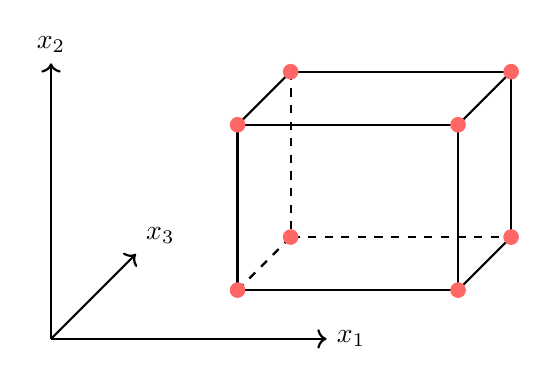
\begin{tikzpicture}[scale = 0.7,
    vertex/.style={circle, fill=red!60, inner sep=2pt},
    edge/.style={thick}
]

% Coordinates of the cuboid
\coordinate (O)   at (3,0.5,-1);
\coordinate (A)   at (7,0.5,-1);
\coordinate (B)   at (7,3.5,-1);
\coordinate (C)   at (3,3.5,-1);

\coordinate (O1)  at (3,0.5,-3.5);
\coordinate (A1)  at (7,0.5,-3.5);
\coordinate (B1)  at (7,3.5,-3.5);
\coordinate (C1)  at (3,3.5,-3.5);

% Coordinate axes
\draw[->, thick] (0,0,0) -- (5,0,0) node[right] {$x_1$};
\draw[->, thick] (0,0,0) -- (0,5,0) node[above]  {$x_2$};
\draw[->, thick] (0,0,0) -- (0,0,-4) node[above right] {$x_3$};

% Cuboid edges
\draw[edge] (O)  -- (A)  -- (B)  -- (C)  -- cycle;
\draw[edge, dashed] (C1) -- (O1) -- (A1);
\draw[edge] (A1) -- (B1) -- (C1);

\draw[edge, dashed] (O)  -- (O1);
\draw[edge] (A)  -- (A1);
\draw[edge] (B)  -- (B1);
\draw[edge] (C)  -- (C1);

% Mark all 8 vertices
\foreach \p in {O,A,B,C,O1,A1,B1,C1}
    \node[vertex] at (\p) {};

% Vertex labels
% \node[below left]  at (O)  {$v_1$};
% \node[below]       at (A)  {$v_2$};
% \node[right]       at (B)  {$v_3$};
% \node[left]        at (C)  {$v_4$};

% \node[left]        at (O1) {$v_5$};
% \node[below right] at (A1) {$v_6$};
% \node[right]       at (B1) {$v_7$};
% \node[left]        at (C1) {$v_8$};

% \node[left]        at (-2,2.5,0) {$P(x_1,x_2,x_3) = \ldots + 5x_1x_2x_3 + \dots$};

\end{tikzpicture}
    \vspace{-5mm}
    \caption{The special case of the Nullstellensatz we use, with $n = 3$: If $P\in \R[x_1,x_2,x_3]$ has degree $3$ and vanishes on all $8$ vertices of some axis-aligned cuboid (in red), then the coefficient of $x_1x_2x_3$ in $P$ must be $0$.}
    \label{fig:CN}
\end{figure}

\begin{proof}[Proof of \Cref{lem:xor-null}]
    For contradiction, assume we have such a monomial $M$. Note that $M$ cannot contain both~$z^+_i=x_i+y_i$ and $z^-_i=x_i-y_i$ for any $i$ because of independence in $G^{(2)}$, as $z^+_i$ and $z^-_i$ are substituted in $P$ as variables with numbers $i$ and $n + i$. For every $z^+_i$ in $M$, we restrict to $x_i = y_i$. For every $z^-_i$ in $M$, we restrict to $x_i \neq y_i$. This restricts the corresponding inputs of $f$ to $0$ and~$1$, respectively. Moreover, since the monomial is independent in $G^{(2)}$, the set of restricted input bits of $f$ forms an independent set in $G$ of size $\deg(P)$. Because $\res_G(f) \geq \deg(P)$, we can extend this restriction to an input $a \in f^{-1}(0)$. We now fix all $x_i$ and $y_i$ that are not part of the above relations in such a way that $x_i \oplus y_i$ agrees with $a_i$, thus also fixing both $z^+_i$ and $z^-_i$. Now, the only $z^+_i$ that are not fixed are exactly the ones appearing in $M$, each of which can independently take a value $z^+_i\in \{0,2\}$. Similarly, the only $z^-_i$ not yet fixed are the ones in $M$, with $z^-_i \in \{-1, 1\}$. Therefore, together with the fixed $z^{\pm}$-variables, these values form a grid that satisfies the conditions of Combinatorial Nullstellensatz (\cref{thm:nullstellensatz}) for the monomial $M$. Thus, there must exist a point on this grid where the polynomial does not vanish, which contradicts the fact that $a \in f^{-1}(0)$.
\end{proof}



\subsection{Rank method and proof of \cref{lem:h-bound}} \label{sec:rank-method}

Here we prove  \Cref{lem:h-bound} by developing a rank argument. For a polynomial $Q$ of degree $d$, we will denote by~$Q^{(d)}$ the \emph{degree-$d$ homogeneous part} of $Q$.
  
\begin{boxdefinition}\label{def:derivative-matrix}
    Let $Q \in \mathbb{R}[x_1,\dots,x_n]$ have degree $d\geq 1$. Define the \emph{first-derivative coefficient matrix} $D_Q$ with rows indexed by $i\in [n]$ and columns indexed by degree-$(d-1)$ monomials in the variables of $Q$.
    The entry for row $i$ and monomial $M$ is 
    \[
        D_Q(i,M)\coloneqq \text{ coefficient of } M \text{ in } \frac{\partial Q^{(d)}}{\partial x_i}.
    \]
\end{boxdefinition}
    Note that by definition, $\rk(D_Q) = \dim \mathrm{span}\left\{ \frac{\partial Q^{(d)}}{\partial x_1},\cdots, \frac{\partial Q^{(d)}}{\partial x_n}  \right\}$.
The crucial property is that 
$D_Q(i,M)\neq 0$ if and only if $x_iM$ is a degree-$d$ monomial of $Q$. In fact, we have $D_Q(i,M) = (r+1)\cdot c$ where $r$ is the exponent of $x_i$ in $M$ and $c$ is the coefficient of $x_iM$ in $Q$.

\begin{boxlemma} \label{lem:sketch-derivative-rank}
    Let $P \in \mathbb{R}[u_1,\cdots,u_k]$ and $A:\mathbb{R}^n\to \mathbb{R}^k$ be a linear map. For $Q(x) \coloneqq P(Ax)$, we have
    \[
        \rk(D_Q)\leq \rk(A)\leq k.
    \]
\end{boxlemma}

\begin{proof}
    Let $d$ be the degree of $Q$ and let $A(x) = (L_1(x),\cdots,L_k(x))$, where $L_j(x) = \sum A_{ji}x_i$. Then, we have $Q^{(d)} = P^{(d)}(L_1(x),\cdots,L_k(x))$. By the chain rule,
    \[
        \frac{\partial Q^{(d)}}{\partial x_i} = \sum_{j=1}^k  \frac{\partial P^{(d)}}{\partial u_j} (Ax)\cdot  \frac{\partial L_j}{\partial x_i}=\sum_{j=1}^k A_{j,i} \cdot \frac{\partial P^{(d)}}{\partial u_j}(Ax).
    \]
    Hence the partial derivatives of $Q^{(d)}$ are linear combinations of $k$ fixed polynomials, with coefficient vectors given by the columns of $A$.
We claim that $\rk(D_Q) \leq \rk(A)$. 
Let $\frac{\partial P^{(d)}}{\partial u_j} (Ax) = \sum_M B_{j,M}M$ where $M$ ranges over all degree-$(d-1)$ monomials in $x_1,\cdots,x_n$. Then 
\[ \frac{\partial Q^{(d)}}{\partial x_i} =\sum_M \left(\sum_{j=1}^k A_{j,i}B_{j,M}\right)M,\]
hence, $D_Q = A^\top B$ and $\rk(D_Q)\leq \rk(A^\top) = \rk(A)\leq k$.
\end{proof}


The next lemma converts a bound on derivative coefficient rank into the existence of either a hitting set or a monomial whose support is an independent set. 

\begin{boxlemma}\label{lem:rank-lower-bound}
    Let \(Q \in \mathbb{R}[x_1,\dots,x_n]\) be a polynomial of degree $d\geq 1$, and let $G$ be a graph on $[n]$.
    If no degree-$d$ monomial of $Q$ is independent in $G$, then
    \[
        h_G(Q)\leq d \cdot \rk(D_Q).
    \]
\end{boxlemma}

 

\begin{proof}
    We show that $D_Q$ has a triangular sub-matrix of size at least $h_G(Q)/d$ (with no zeros on the diagonal). View each monomial $M$ as a multiset of its $d$ variables.
    Define $E(M)$ as the number of edges of $G$ among the variables appearing in $M$:
    \[
        E(M) \coloneqq \#\bigl\{\{x_i,x_j\} \subseteq M : i \sim_G j\bigr\}.
    \]
    Note that a variable with multiplicity $k\geq 2$ in $M$ contributes $\binom{k}{2}$ edges to $E(M)$. Thus, $M$ is independent in $G$ if and only if $E(M) = 0$. Hence, by our hypothesis, every degree-$d$ monomial of $Q$ has $E(M) \geq 1$.

    \paragraph{The pivoting step.}
    Suppose $I\subseteq [n]$ is a set of variables with $|I| < h_G(Q)$. Then, some degree-$d$ monomial avoids $N_G(I)$.
    Choose one such monomial $M$ which minimises $E(M)$, and pick a variable $x_i$ of $M$ with
    \[
        E(M/x_i) < E(M).
    \]
    Such an $x_i$ exists because $E(M)\geq 1$.
    Let $M' \coloneqq M/x_i$. Then:
    \begin{enumerate}
        \item[(a)] We have $D_Q(i, M') \neq 0$, because $M'x_i = M$ is a top-degree monomial of $Q$.
        \item[(b)] Moreover, $i \notin N_G(I)$, since we picked $M = M'x_i$ to avoid $N_G(I)$.
        \item[(c)] Finally, for every $j$ with $D_Q(j, M') \neq 0$, we have $j\in N_G(\supp(M')\cup I)$. If not, then $x_jM'$ would be a top-degree monomial in $Q$ avoiding $N_G(I)$. But since $j\not\in N_G(\supp(M'))$, we would have $E(x_jM') < E(M)$, contradicting minimality of $E(M)$.
    \end{enumerate}
    
    \paragraph{Building a triangular sub-matrix.}
    We will construct a triangular sub-matrix (with no zero on the diagonal) in $D_Q$, by repeatedly using the pivoting step to pick rows $i_1,i_2,\dots$ and columns corresponding to degree-$(d-1)$ monomials $M'_1,M'_2,\dots$ in $Q$.
    
    For $t\geq 1$, suppose we have already found pivot rows $i_1,\dots, i_{t-1}$ and monomials $M'_1,\dots, M'_{t-1}$. Set
    \[
        I_{t-1} \coloneqq \supp(M'_1x_{i_1})\cup \supp(M'_2x_{i_2})\cup \cdots \cup \supp(M'_{t-1}x_{i_{t-1}}).
    \]
    As long as $|I_{t-1}| < h_G(Q)$, the pivoting step applied to $I_{t-1}$ produces a degree-$d$ monomial $M_t$, a pivot row $i_t\in \supp(M_t)$ and a column $M'_t \coloneqq M_t/x_{i_t}$ which satisfy the  three properties listed above.
    We now show that the new sub-matrix of $D_Q$ induced by rows $\{i_1,\dots,i_t\}$ and columns corresponding to $\{M'_1,\dots, M'_t\}$ is again triangular (after reordering), with non-zero diagonal:
    
    Fix $s < t$ and consider entry $D_Q(i_t, M'_s)$. By property (c) of the $s$-th pivoting step, this entry can be non-zero only if $i_t\in N_G(\supp(M'_s)\cup I_{s-1}) \subseteq N_G(I_{t-1})$. But property (b) of the $t$-th pivoting step guarantees $i_t\notin N_G(I_{t-1})$. Hence $D_Q(i_t, M'_s) = 0$ for all $s<t$, while $D_Q(i_t,M'_t)\neq 0$ (property (a) of the $t$-th pivoting step).

    The process terminates only when $h_G(Q) \leq |I_t|$. Since $|I_t|\leq \sum_{i = 1}^t|\supp(M'_ix_i)| = td$, we get a triangular sub-matrix of size at least $h_G(Q)/d$, as desired.
\end{proof}
 
\begin{proof}[Proof of \Cref{lem:h-bound}]
    By \Cref{lem:sketch-derivative-rank}, we have $\rk(D_Q) \leq \rk(A) \leq k$.  By \Cref{lem:rank-lower-bound}, $h_G(Q)\leq d\cdot \rk(D_Q)$. The result follows from combining the two bounds.
\end{proof}


\section{Boolean closures (\cref{thm:main-ext})}

In this section we will extend our lower bounds to the boolean closure of support-sketches. The proof mirrors the main argument in \cite{FGHH25}, and we will only make explicit the parts that deviate from it.

\medskip

Let $A \in \{0,1\}^{n\times n}$ be a matrix. For an index $i\in [n]$, we denote by $A_i$ the $i$-th row of $A$. For a permutation $\pi$ acting on $[n]$, we denote by $A_{\pi}$ the matrix with rows $A_{\pi(1)},A_{\pi(2)},\dots, A_{\pi(n)}$.

\begin{boxdefinition}[Minor-Closure]
    We say that a family $\mathcal{F}$ of boolean functions on $\{0,1\}^\ast$ is \emph{minor-closed}, if for any $f\colon\{0,1\}^n\to\{0,1\}$ in $\mathcal{F}$ and any affine function $A\colon\{0,1\}^m\to \{0,1\}^n$ with $m\geq n$, the composition $f\circ A$ is also in $\mathcal{F}$.
\end{boxdefinition}


Since $\{0,1\}^n\times \{0,1\}^n \cong \{0,1\}^{2n}$, this definition naturally extends to two-party functions.

\begin{lemma}\label{lem:SK-closed}
    The family of functions for which $\sk_0 \leq k + d$ is minor-closed.
\end{lemma}

\begin{proof}
    Note that affine change of variables turns linear sketches into affine sketches. However, the additive constant can be absorbed in the polynomial, whose degree is unchanged.
\end{proof}

\begin{boxdefinition}[Stackability]
    We say that a function $f$ on boolean square matrices is \emph{stackable} if
    \[
        \forall\, X\in\{0,1\}^{n\times n}\colon\quad
        f(X) = f\left(
        \begin{matrix}
            X & 0 \\
            X & 0      
        \end{matrix}
        \right).
    \]
\end{boxdefinition}

\begin{example}
    Any property of boolean matrices that only depends on the rank of the matrix is stackable. The same is true for support-rank and sign-rank.
\end{example}

\begin{boxdefinition}[Stability]
    We say that a function $f\colon\{0,1\}^n\times \{0,1\}^n\to\{0,1\}$ is $t$-\emph{stable} if there do not exist inputs $x_1,y_1\dots, x_t,y_t\in \{0,1\}^n$ such that for all $1\leq i,j\leq t$ we have
    \[
        f(x_i, y_j) = 1\iff i \geq j.
    \]
    We call a family of functions $\mathcal{F}$ \emph{stable} if there exists a $t\geq 2$ such that every $f\in \mathcal{F}$ is $t$-stable.
\end{boxdefinition}

If a function is $t$-stable, then clearly it is also $(t+1)$-stable.

\begin{boxlemma}\label{lem:stable-supp}
    Any function $f\colon\{0,1\}^n\times \{0,1\}^n\to\{0,1\}$ is $t$-stable for both
    \[
        t = \rk_0(f)+1 \quad\text{and}\quad t = \rk_0(\neg f)+2.
    \]
\end{boxlemma}
\begin{proof}
    Assume that $f$ is not $t$-stable, witnessed by $x_i$ and $y_i$ with $i\in[t]$. Let $M\in\R^{2^n\times 2^n}$ with $\rk(M) = \rk_0(f)$ and the same support-pattern as $f$. The sub-matrix of $M$ induced by the $x_i$ and $y_i$ is a triangular matrix, and thus has rank $t$. We conclude that $t \leq \rk(M) \leq \rk_0(f)$. Similarly, $t\leq \rk_0(\neg f) + 1$, since the rank of the induced sub-matrix in $\neg M$ is $t-1$.
\end{proof}

\begin{lemma}
    For a number of sketches $k$ and degree $d$, a function with $\sk_0 \leq k + d$ is $O(k + d)^d$-stable.
\end{lemma}
    
\begin{proof}
    We know that $\rk_0(f) \leq O(k+d)^d$ by
    \Cref{lem:sketch-to-rank}. The statement thus follows directly from \cref{lem:stable-supp}.
\end{proof}

\begin{boxdefinition}[Row-Swap]
    Given matrices $A,B \in \{0,1\}^{n\times n}$, a \emph{row-swap} consists of picking a transposition $\pi = (i,i+1)\in S_n$ of consecutive indices, and replacing $A,B$ with $A_\pi,B_\pi$ respectively. The \emph{type} of this row-swap is the tuple $(A_i,A_{i+1},B_i,B_{i+1}) \in \{0,1\}^{4n}$.
\end{boxdefinition}

\begin{boxdefinition}[Row-Shuffle-Invariance]
    Let $f\colon \{0,1\}^{n\times n} \times \{0,1\}^{n\times n}\to \{0,1\}$ and $\Delta \subseteq \{0,1\}^{4n}$. We say $f$ is $\Delta$\emph{-row-shuffle-invariant} if it is invariant under applying, to its two inputs, any row-swap with type in $\Delta$. 
    
    For $f \colon \{0, 1\}^{m \times m} \times \{0, 1\}^{m \times m} \to \{0, 1\}$ and $\Delta \subseteq \{0, 1\}^{4n}, m \geq n$, we say that $f$ is $\Delta$-row-shuffle-invariant if it is invariant under all row swaps of types $(a0^{m-n}, b0^{m - n}, c0^{m - n}, d0^{m - n})$ for $(a, b, c, d) \in \Delta$. We say $f$ is \emph{row-shuffle-invariant} if it is invariant under row-swaps of all possible types.
\end{boxdefinition}

Note that a function $f$ is row-shuffle-invariant exactly if it is invariant under shuffling the rows of the two input matrices with the same, arbitrary permutation. We similarly define \emph{column-shuffle-invariance}. If such a function is both row-shuffle-invariant and column-shuffle-invariant, we call it \emph{shuffle-invariant}.

\begin{boxdefinition}[$\xor$-Invariance]
    Let $f\colon \{0,1\}^{n\times n} \times \{0,1\}^{n\times n}\to \{0,1\}$. We say $f$ is $\xor$\emph{-invariant}, if for any $x, y, z \in \{0, 1\}^{n \times n}$ it holds that $f(x, y) = f(x \oplus z, y \oplus z)$.
\end{boxdefinition}

\begin{boxdefinition}
    Let $\mathcal{Q}$ be a family of two-party functions. We define its \emph{boolean closure} $\overline{\mathcal{Q}}$ as the family of all functions $f\colon\{0,1\}^n\times\{0,1\}^n\to\{0,1\}$ for which the following holds: There exists a constant $s\in\N$, such that for all $n\in\N$ we have
    \[
        \forall\, x,y\in\{0,1\}^n:\quad
        f(x,y) = \Gamma\big(q_1(x,y),\ q_2(x,y),\ \dots\ ,\ q_s(x,y)\big),
    \]
    for some $\Gamma:\{0,1\}^s\to\{0,1\}$ and some $q_1,q_2,\dots,q_s\in \mathcal{Q}$ (which can both depend on $n$).
\end{boxdefinition}

Informally, the following theorem states that if an $f\in\overline{\mathcal{Q}}$ exhibits certain symmetries, then we can express $f$ as a uniform boolean combination of some functions in $\mathcal{Q}$ that share the same symmetries as $f$.

\begin{boxtheorem}\label{thm:query-inv}
    Let $\mathcal{Q}$ be a stable, minor-closed family of boolean two-party functions on bit-strings. Let the function $f\colon \{0,1\}^{n\times n} \to \{0,1\}$ be shuffle-invariant and stackable.
    
    If $f\circ \xor\in \overline{\mathcal{Q}}$, then there exists a fixed function $\Gamma\colon \{0,1\}^s\to \{0,1\}$ such that for all $n\in\mathbb{N}$, there are shuffle-invariant $\xor$-functions $q_1,q_2, \dots, q_s \in \mathcal{Q}$ satisfying
    \[
        \forall\, x,y\in \{0,1\}^{n\times n}\ \colon\quad
        (f\circ \xor)(x,y) = \Gamma\big(q_1(x,y), \dots, q_s(x,y)\big).
    \]
\end{boxtheorem}

We prove \Cref{thm:query-inv} by establishing the following incremental results:

\paragraph{Part 1}
The result holds if the $q_i\in \mathcal{Q}$ are allowed to be arbitrary. 

\paragraph{Part 2}
Using that $f$ is row-shuffle-invariant, the $q_i$ can be made $\Delta_n$-row-shuffle-invariant with
\[
    \Delta_n = \{(a,b,c,d) \in \{0,1\}^{4n}\mid a = c \text { or } b = d\}.
\]

\paragraph{Part 3}
Using that $\mathcal{Q}$ is stable, the $q_i$ can be made fully row-shuffle-invariant.

\paragraph{Part 4}
Using that $f$ is column-shuffle-invariant, the $q_i$ can also be made column-shuffle invariant.

\paragraph{Part 5}
Using that $f$ is stackable, the $q_i$ can further be made $\xor$-invariant.

\medskip


 \medskip

Part 1 holds by the definition of $\overline{\mathcal{Q}}$.
For Part 2, we refer the reader to \cite{FGHH25}, Proposition 41. The only difference, apart from notational convention, is that we assume $\mathcal{Q}$ to be minor-closed, which is more restrictive than their notion of ``query family''. However, this does not affect the proofs they give. 

 Below we refer to a dimension $n$ being ($\Delta$-)shuffle-invariant meaning that $q_i$ for this dimension are ($\Delta$-)shuffle-invariant. We present the reformulation of the statement from \cite{FGHH25} and explain the differences in notation below.

\begin{boxlemma}[Proposition 41 in \cite{FGHH25}]
\label{lm:part2}
    Let $a \in \{0, 1\}^n$, $\Delta_a^i = \{(a^i, \ast, a^i, \ast)\} \cup \{(\ast, a^i, \ast, a^i)\}$, $B \subseteq \{0, 1\}^n$ and $\Delta^i = \bigcup_{b \in B}\Delta_{b}^{i}$. If for every $n$, $\Delta^i$-row-shuffle invariance holds for dimension $n \cdot i$, then $\Delta^i\cup \Delta_a^i$-row-shuffle invariance also holds for every $n \cdot i$.
\end{boxlemma}
\begin{proof}[Notational differences]
    The proof in \cite{FGHH25} deals with rectangular matrices; one can keep the matrices square by padding them with copies of $a$, which does not affect the proof. This is because by construction, the padded rows always coincide outside of the embedded smaller matrices, so swapping shorter rows (\emph{dominoes}) equal to $a \in \{0, 1\}^n$ in \cite{FGHH25} is the same as our swapping rows from $\{0, 1\}^{n \cdot i}$ with swap type in $\Delta_a^i$. The rest of the proof carries over verbatim.
\end{proof}

Applying \cref{lm:part2} repeatedly for every $a$ proves part 2.

\medskip

The proof of part 3 in \cite{FGHH25} uses the previously established ``inner-permutation-invariance'', which is particular to the $(4,4)$-$\HD$ problem. However, this assumption is not necessary and we give an alternative proof below, which also significantly simplifies this part of the argument in \cite{FGHH25}.


\begin{proof}[Proof of Part 3]
    We can assume that all dimensions $n$ are already $\Delta_n$-shuffle-invariant. 
    
    For a given $n$, we use \cref{alg:symmetrisation2} to make it fully shuffle-invariant. During its runtime, the algorithm extends the sets of shuffle invariance for $n$ as well as for some bounded number of dimensions greater than $n$. We specify later what the extension procedure itself looks like; the algorithm describes the order of applying it to different dimensions. Let $t\geq 2$ be such that $\mathcal{Q}$ is $t$-stable.

    \begin{algorithm}
        \begin{algorithmic}
            \State {$\Delta = \varnothing$}
            \For {$0 \leq i < 2^{4n}$}
                \State {Let $p_i$ be the $4n$-bit representation of $i$}
                % \State {$\Delta \gets \Delta \cup p_i$}
                \For {$j \gets n + 2t \cdot (2^{4n} - i - 1)$; $j \geq n$; $j \mathrel{{-}{=}} 2t$}
                    \State {Make $j$ invariant wrt $\Delta \cup \Delta_j \cup p_i$}
                \EndFor
                \State {$\Delta \gets \Delta \cup p_i$}
            \EndFor
        \end{algorithmic}
        \caption{Symmetrisation procedure}
        \label{alg:symmetrisation2}
    \end{algorithm}

    Note that when the algorithm tries to ensure the shuffle invariance for some dimension $m$ with respect to $\Delta \cup \Delta_m \cup p$, we have already ensured that $m + 2t$ is invariant with respect to $\Delta \cup \Delta_{m + 2t}$. We now need to show that we can indeed extend the shuffle invariance for $m$ in such a case, and this will prove the correctness of the procedure.

    Let $p = (a, b, c, d)$ and let us pad each row with $0$s according to the dimension $m$. Consider the embedding $\phi\colon \{0,1\}^{m\times m} \to \{0,1\}^{(m+2t)\times (m+2t)}$ that adds to the input matrix $t$ many rows equal to $a$ and $t$ many rows equal to $d$, padding each row with $2t$ trailing zeros. Concretely, for all $i\in [m+2t]$, we have
    \[
        \phi(x)_i = \begin{cases}
            x_i\ 0^{2t}&\text{if } i \leq m,\\
            a\ 0^{2t}&\text{if } m < i \leq m+t,\\
            d\ 0^{2t}&\text{if } m+t < i \leq m+2t.
        \end{cases}
    \]
    Consider $\Gamma$ and $q'_i$ satisfying \cref{eq:Gamma} for input matrices of size $(m+2t)\times (m+2t)$ such that each $q'_i$ is $\Delta \cup \Delta_{m + 2t}$-row-shuffle-invariant.
    Now define $q_i$ by
    \[
        \forall x,y\in\{0,1\}^{m\times m}:\quad
        q_i(x,y) = q'_i(\phi(x),\phi(y)).
    \]
    Since $q_i$ is an affine restriction of $q'_i$ and $\mathcal{Q}$ is minor-closed, we have $q_i\in \mathcal{Q}$. Moreover, $q_i$ inherits $\Delta \cup \Delta_m$-shuffle-invariance from $q'_i$.
    We now prove that each $q_i$ is $p$-row-shuffle-invariant as well. If not, then for some $i$ there exist $x,y\in\{0,1\}^{m\times m}$ and a transposition $\pi = (j,j+1) \in S_m$ with $q_i(x,y) \neq q_i(x_\pi,y_\pi)$ and
    \begin{alignat*}{2}
        x_j &= a,\quad y_j &&= c,\\
        x_{j+1} &= b,\quad y_{j+1} &&= d.
    \end{alignat*}
    
    For all $k\in [t+1]$, we now define the matrix
    $x(k)\in\{0,1\}^{(m+2t)\times (m+2t)}$ as follows: The rows indexed $j$ and $j+1$ are replaced by $2t+2$ alternating copies of $a$ and $d$. Then, the $k$-th copy of $d$ we just added is replaced by $b$. Finally, all rows are padded with $2t$ trailing zeros. Similarly define $y(k)$, where instead the $k$-th copy of $a$ is replaced by $c$. Now note that, by $\Delta$-row-shuffle-invariance, for $u,v\in [t+1]$ we have
    \[
        q'_i(x'(u),y'(v)) = \begin{cases}
            q'_i(\phi(x),\phi(y)) \quad = q_i(x,y) ,&\text{if } u \geq v\\
            q'_i(\phi(x_\pi),\phi(y_\pi)) = q_i(x_\pi,y_\pi),&\text{if } u < v.
        \end{cases}
    \]
    But this contradicts $t$-stability of $\mathcal{Q}$. The matrices in question are illustrated in \cref{fig:stable}.
\end{proof}

\begin{figure}[ht]
        \centering
        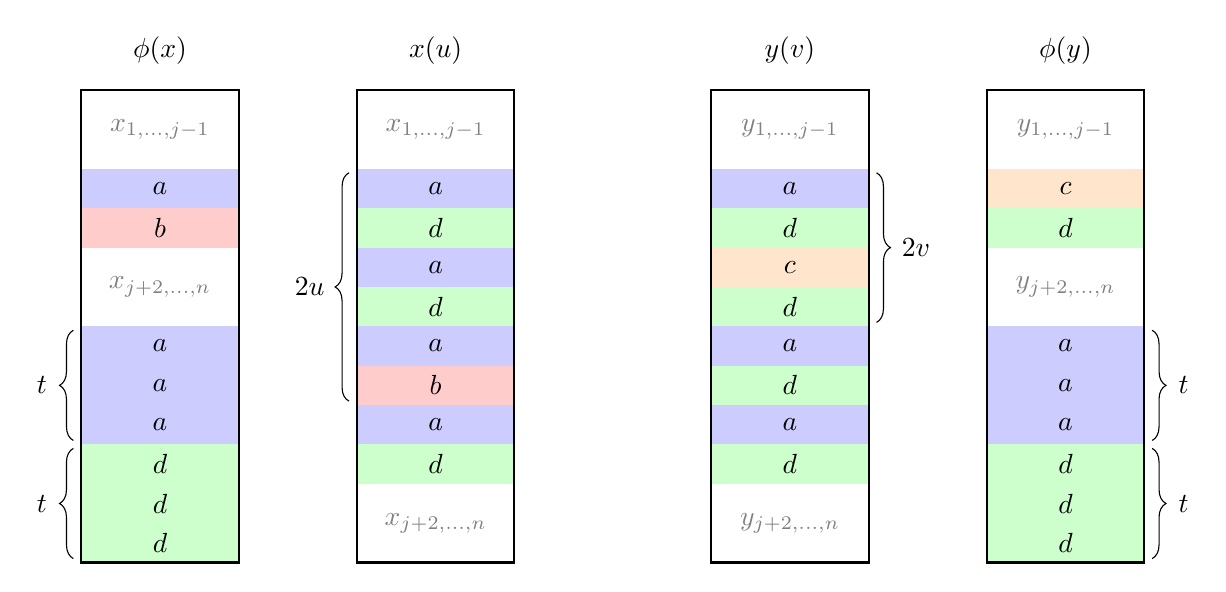
\begin{tikzpicture}[scale = 0.5]
		
	\fill[blue!20] (0,10) rectangle (4,9);
        \node at (2, 9.5) {$a$};
        
        \fill[red!20] (0, 9) rectangle (4,8);
        \node at (2, 8.5) {$b$};
    
        \fill[blue!20] (0,6) rectangle (4,3);
        \node at (2, 5.5) {$a$};
        \node at (2, 4.5) {$a$};
        \node at (2, 3.5) {$a$};
        
        \fill[green!20] (0,3) rectangle (4,0);
        \node at (2, 2.5) {$d$};
        \node at (2, 1.5) {$d$};
        \node at (2, 0.5) {$d$};

        \draw [decorate, decoration={brace, amplitude=5pt, raise=1mm}] (0,0.1) -- (0,2.9) node[midway, xshift=-5mm]{$t$};
        \draw [decorate, decoration={brace, amplitude=5pt, raise=1mm}] (0,3.1) -- (0,5.9) node[midway, xshift=-5mm]{$t$};

        \draw[thick] (0,0) rectangle (4,12);
        \node at (2, 13) {$\phi(x)$};

        \node[gray] at (2, 11) {$x_{1,\dots, j-1}$};
        \node[gray] at (2, 7) {$x_{j+2,\dots, n}$};
        

        \tikzset{shift={(7, 0)}}

        \fill[blue!20] (0,10) rectangle (4,9);
        \node at (2, 9.5) {$a$};
        \fill[green!20] (0, 9) rectangle (4,8);
        \node at (2, 8.5) {$d$};
        \fill[blue!20] (0,8) rectangle (4,7);
        \node at (2, 7.5) {$a$};
        \fill[green!20] (0, 7) rectangle (4,6);
        \node at (2, 6.5) {$d$};
        \fill[blue!20] (0,6) rectangle (4,5);
        \node at (2, 5.5) {$a$};
        \fill[red!20] (0, 5) rectangle (4,4);
        \node at (2, 4.5) {$b$};
        \fill[blue!20] (0,4) rectangle (4,3);
        \node at (2, 3.5) {$a$};
        \fill[green!20] (0, 3) rectangle (4,2);
        \node at (2, 2.5) {$d$};

        \draw [decorate, decoration={brace, amplitude=5pt, raise=1mm}] (0,4.1) -- (0,9.9) node[midway, xshift=-6mm]{$2u$};
	
	\draw[thick] (0,0) rectangle (4,12);
        \node at (2, 13) {$x(u)$};

        \node[gray] at (2, 11) {$x_{1,\dots, j-1}$};
        \node[gray] at (2, 1) {$x_{j+2,\dots, n}$};


        \tikzset{shift={(9, 0)}}

        \fill[blue!20] (0,10) rectangle (4,9);
        \node at (2, 9.5) {$a$};
        \fill[green!20] (0, 9) rectangle (4,8);
        \node at (2, 8.5) {$d$};
        \fill[orange!20] (0,8) rectangle (4,7);
        \node at (2, 7.5) {$c$};
        \fill[green!20] (0, 7) rectangle (4,6);
        \node at (2, 6.5) {$d$};
        \fill[blue!20] (0,6) rectangle (4,5);
        \node at (2, 5.5) {$a$};
        \fill[green!20] (0, 5) rectangle (4,4);
        \node at (2, 4.5) {$d$};
        \fill[blue!20] (0,4) rectangle (4,3);
        \node at (2, 3.5) {$a$};
        \fill[green!20] (0, 3) rectangle (4,2);
        \node at (2, 2.5) {$d$};

        \draw [decorate, decoration={brace, amplitude=5pt, raise=1mm}] (4,9.9) -- (4,6.1) node[midway, xshift=6mm]{$2v$};

        \draw[thick] (0,0) rectangle (4,12);
        \node at (2, 13) {$y(v)$};

        \node[gray] at (2, 11) {$y_{1,\dots, j-1}$};
        \node[gray] at (2, 1) {$y_{j+2,\dots, n}$};
        

        \tikzset{shift={(7, 0)}}

        \fill[orange!20] (0,10) rectangle (4,9);
        \node at (2, 9.5) {$c$};
        \fill[green!20] (0, 9) rectangle (4,8);
        \node at (2, 8.5) {$d$};
        
        \fill[blue!20] (0,6) rectangle (4,3);
        \node at (2, 5.5) {$a$};
        \node at (2, 4.5) {$a$};
        \node at (2, 3.5) {$a$};
        \fill[green!20] (0,3) rectangle (4,0);
        \node at (2, 2.5) {$d$};
        \node at (2, 1.5) {$d$};
        \node at (2, 0.5) {$d$};

        \draw [decorate, decoration={brace, amplitude=5pt, raise=1mm}] (4,2.9) -- (4,0.1) node[midway, xshift=5mm]{$t$};
        \draw [decorate, decoration={brace, amplitude=5pt, raise=1mm}] (4,5.9) -- (4,3.1) node[midway, xshift=5mm]{$t$};
	
	\draw[thick] (0,0) rectangle (4,12);
        \node at (2, 13) {$\phi(y)$};

        \node[gray] at (2, 11) {$y_{1,\dots, j-1}$};
        \node[gray] at (2, 7) {$y_{j+2,\dots, n}$};
	
\end{tikzpicture}
        \caption{If $u \geq v$, the matrices $\phi(u),\phi(u)$ can be obtained from matrices $x(u),y(v)$ with row-swaps of type $(a0^{2t},\ast,a0^{2t},\ast)$ and $(d0^{2t},\ast,d0^{2t},\ast)$, which are both in $\Delta_{m + 2t}$. If $u < v$, the same is true with $\phi(x_\pi),\phi(y_\pi)$ instead.}
        \label{fig:stable}
    \end{figure}

\begin{proof}[Proof of Part 4]
    Assume that $f$ is also column-shuffle-invariant. For any function $g\colon \{0,1\}^{n\times n}\times \{0,1\}^{n\times n}\to\{0,1\}$, define the function $g^T$ by
    \[
        \forall x,y\in\{0,1\}^{n\times n}:\quad
        g^T(x,y) = g(x^T,y^T).
    \]
    Note that since $f$ is column-shuffle-invariant, $f^T$ is row-shuffle-invariant. Thus, by the previous part, there exist $\Gamma$ and row-shuffle-invariant $q_i$ such that
    \[
        (f\circ \xor)(x,y) = (f^T\circ \xor)(x^T,y^T) = \Gamma\big(q_1(x^T,y^T),\ \dots,\ q_s(x^T,y^T)\big) = \Gamma\big(q_1^T(x,y),\ \dots,\ q_s^T(x,y)\big).
    \]
    But note that for each $i$, the function $q_i^T$ is column-shuffle-invariant. Since transposition of the input is just a reordering of the variables, we also have $q_i^T \in \mathcal{Q}$ by minor-closure. We conclude that part 3 also holds if ``row-shuffle-invariant'' is replaced by ``column-shuffle-invariant''. To see why we can guarantee both properties simultaneously, it suffices to notice that the construction in parts 2 and 3 preserves column-shuffle-invariance.
\end{proof}

\begin{proof}[Proof of Part 5]
    Assume that $f$ is stackable. For each $i\in [2^n]$, let $\Psi(i)\in \{0,1\}^{n\times n}$ be the matrix with all rows equal to the binary expansion of $i-1$.
    For $x\in\{0,1\}^{n\times n}$, denote by $\Phi(x)\in \{0,1\}^{n2^n \times n2^n}$ the matrix obtained by stacking the matrices
    \[
        x\oplus \Psi(1),\ x\oplus \Psi(2),\ \dots,\ x \oplus \Psi(2^n)
    \]
    on top of each other, padding each row with $n(2^n-1)$ many trailing zeros, as illustrated in \Cref{fig:stack}. We have
    \[
        \forall x,y\in\{0,1\}^{n\times n}:\quad 
        (f\circ \xor)(\Phi(x),\Phi(y)) = (f\circ \xor)(x,y).
    \]
    Using the result from the previous part, for matrices of size $n2^n \times n2^n$, there are $\Gamma$ and $q'_i$ for which
    \[
        \forall x,y\in \{0,1\}^{n\times n}\ \colon\quad
        (f\circ \xor)(x,y) = \Gamma\big(q'_1\big(\Phi(x),\Phi(y)\big),\ \dots,\ q'_s\big(\Phi(x),\Phi(y)\big)\big),\tag{$\ast$}\label{eq:Gamma}
    \]
    where each $q'_i$ is row-shuffle invariant and column-shuffle-invariant. Define $q_i$ by
    \[
        \forall x,y\in \{0,1\}^{n\times n}:\quad
        q_i(x,y) = q'_i\big(\Phi(x), \Phi(y)\big).
    \]
    Since $q_i$ is an affine restriction of $q'_i$, we also have $Q_i\in \mathcal{Q}$ by minor-closure. Note that $q_i$ inherits shuffle-invariance from $q'_i$. Moreover, for any $z\in \{0,1\}^{n\times n}$, the matrix $\Phi(x\oplus z)$ can be obtained from $\Phi(x)$ by permuting its rows. Thus, each $q_i$ is also $\xor$-invariant, as desired.
\end{proof}

\begin{figure}
    \centering
    
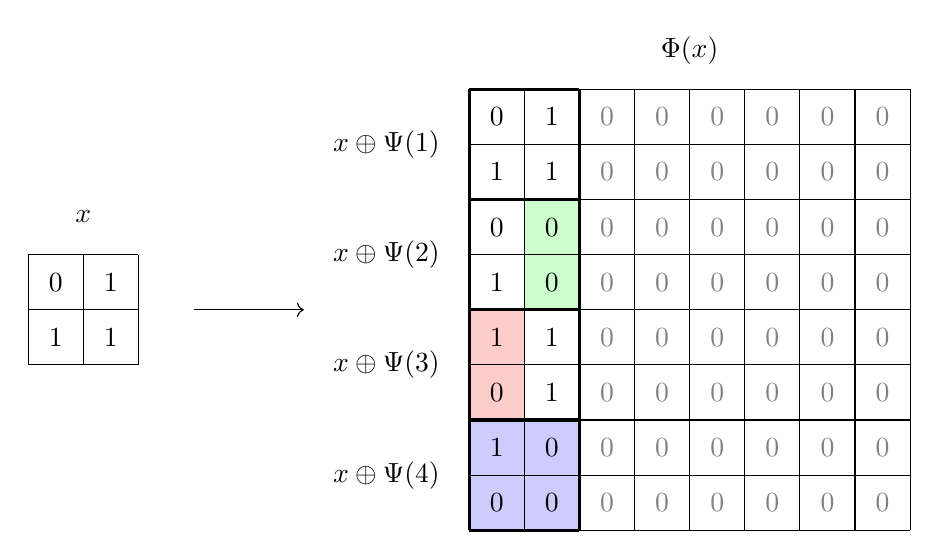
\begin{tikzpicture}[scale=0.7]

\fill[green!20] (5,0) rectangle (6, 2);
\fill[red!20] (4,-2) rectangle (5,0);
\fill[blue!20] (4,-4) rectangle (6,-2);

% Matrix grid
\draw (-4,-1) grid (-2,1);
\draw (4,-4) grid (12,4);

\draw[->] (-1,0) -- (1,0);

\node at (-3,1.7) {$x$};
\node at (8,4.7) {$\Phi(x)$};

\node at (2.5, 3) {$x\oplus\Psi(1)$};
\node at (2.5, 1) {$x\oplus\Psi(2)$};
\node at (2.5, -1) {$x\oplus\Psi(3)$};
\node at (2.5, -3) {$x\oplus\Psi(4)$};


% Matrix entries
\node at (-3.5, 0.5) {0};
\node at (-2.5, 0.5) {1};
\node at (-3.5,-0.5) {1};
\node at (-2.5,-0.5) {1};

\node at (4.5, 3.5) {0};
\node at (5.5, 3.5) {1};
\node at (4.5, 2.5) {1};
\node at (5.5, 2.5) {1};

\node at (4.5, 1.5) {0};
\node at (5.5, 1.5) {0};
\node at (4.5, 0.5) {1};
\node at (5.5, 0.5) {0};

\node at (4.5,-0.5) {1};
\node at (5.5,-0.5) {1};
\node at (4.5,-1.5) {0};
\node at (5.5,-1.5) {1};

\node at (4.5,-2.5) {1};
\node at (5.5,-2.5) {0};
\node at (4.5,-3.5) {0};
\node at (5.5,-3.5) {0};

\node[text=gray] at (6.5, 3.5) {0};
\node[text=gray] at (7.5, 3.5) {0};
\node[text=gray] at (8.5, 3.5) {0};
\node[text=gray] at (9.5, 3.5) {0};
\node[text=gray] at (10.5, 3.5) {0};
\node[text=gray] at (11.5, 3.5) {0};

\node[text=gray] at (6.5, 2.5) {0};
\node[text=gray] at (7.5, 2.5) {0};
\node[text=gray] at (8.5, 2.5) {0};
\node[text=gray] at (9.5, 2.5) {0};
\node[text=gray] at (10.5, 2.5) {0};
\node[text=gray] at (11.5, 2.5) {0};

\node[text=gray] at (6.5, 1.5) {0};
\node[text=gray] at (7.5, 1.5) {0};
\node[text=gray] at (8.5, 1.5) {0};
\node[text=gray] at (9.5, 1.5) {0};
\node[text=gray] at (10.5, 1.5) {0};
\node[text=gray] at (11.5, 1.5) {0};

\node[text=gray] at (6.5, 0.5) {0};
\node[text=gray] at (7.5, 0.5) {0};
\node[text=gray] at (8.5, 0.5) {0};
\node[text=gray] at (9.5, 0.5) {0};
\node[text=gray] at (10.5, 0.5) {0};
\node[text=gray] at (11.5, 0.5) {0};

\node[text=gray] at (6.5, -0.5) {0};
\node[text=gray] at (7.5, -0.5) {0};
\node[text=gray] at (8.5, -0.5) {0};
\node[text=gray] at (9.5, -0.5) {0};
\node[text=gray] at (10.5, -0.5) {0};
\node[text=gray] at (11.5, -0.5) {0};

\node[text=gray] at (6.5, -1.5) {0};
\node[text=gray] at (7.5, -1.5) {0};
\node[text=gray] at (8.5, -1.5) {0};
\node[text=gray] at (9.5, -1.5) {0};
\node[text=gray] at (10.5, -1.5) {0};
\node[text=gray] at (11.5, -1.5) {0};

\node[text=gray] at (6.5, -2.5) {0};
\node[text=gray] at (7.5, -2.5) {0};
\node[text=gray] at (8.5, -2.5) {0};
\node[text=gray] at (9.5, -2.5) {0};
\node[text=gray] at (10.5, -2.5) {0};
\node[text=gray] at (11.5, -2.5) {0};

\node[text=gray] at (6.5, -3.5) {0};
\node[text=gray] at (7.5, -3.5) {0};
\node[text=gray] at (8.5, -3.5) {0};
\node[text=gray] at (9.5, -3.5) {0};
\node[text=gray] at (10.5, -3.5) {0};
\node[text=gray] at (11.5, -3.5) {0};

\draw[step=2, very thick] (4,-4) grid (6,4);

\end{tikzpicture}
    \caption{For every subset $C$ of columns of $x$, the stack in $\Phi(x)$ contains a copy of $x$ with all bits in $C$ flipped (highlighted). The rows of $\Phi(x)$ are padded with zeros to make the matrix square.}
    \label{fig:stack}
\end{figure}

\begin{boxdefinition}[Promise-Rank]
    For some integer $2\leq t\leq n$, we define the partial function $\PRank^t_{>1}\colon\{0,1\}^{n\times n}\to\{0,1,\ast\}$ as follows: For any $x\in \{0,1\}^{n\times n}$,
    \begin{itemize}
        \item if the $1$s in $x$ form a $t \times t$ combinatorial rectangle, then $\PRank^t_{>1}(x) = 0$, else
        \item if the $1$s in $x$ form a $t \times t$ combinatorial rectangle with a $1\times 1$ hole, then $\PRank^t_{>1}(x) = 1$,
        \item else $\PRank^t_{>1}(x) = \ast$ is unspecified.
    \end{itemize}
\end{boxdefinition}

This function is essentially the same as $\Rank_{>1}$, but with the promise that the 1s of the input form a $t\times t$ rectangle, possibly with a single entry missing. Note that for this function, all yes-inputs and all no-inputs are in the same orbit of the symmetry group generated by shuffle-invariance. See \Cref{fig:promise}.

\begin{figure}
    \centering
    
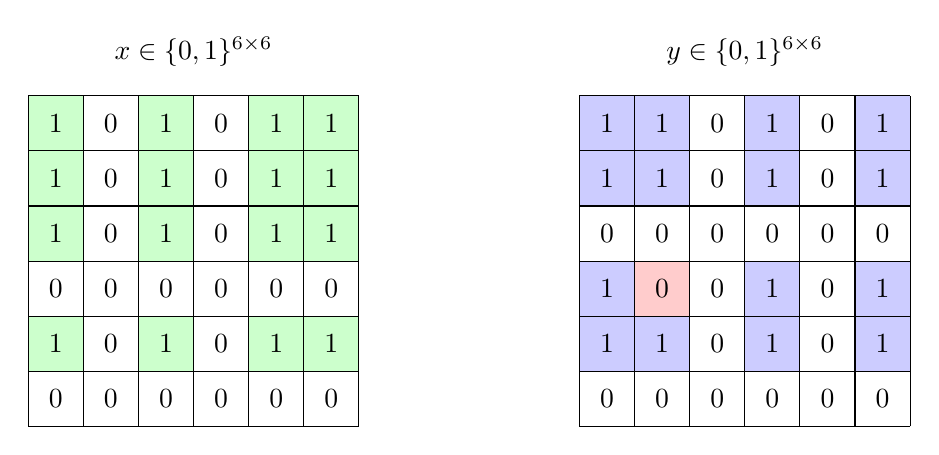
\begin{tikzpicture}[scale=0.7]

\node at (-5, 3.8) {$x\in\{0,1\}^{6\times 6}$};
\node at (5, 3.8) {$y\in\{0,1\}^{6\times 6}$};

\fill[green!20] (-8,-2) rectangle (-7,-1);
\fill[green!20] (-6,-2) rectangle (-5,-1);
\fill[green!20] (-4,-2) rectangle (-3,-1);
\fill[green!20] (-3,-2) rectangle (-2,-1);

\fill[green!20] (-8,-0) rectangle (-7,1);
\fill[green!20] (-6,-0) rectangle (-5,1);
\fill[green!20] (-4,-0) rectangle (-3,1);
\fill[green!20] (-3,-0) rectangle (-2,1);

\fill[green!20] (-8,1) rectangle (-7,2);
\fill[green!20] (-6,1) rectangle (-5,2);
\fill[green!20] (-4,1) rectangle (-3,2);
\fill[green!20] (-3,1) rectangle (-2,2);

\fill[green!20] (-8,2) rectangle (-7,3);
\fill[green!20] (-6,2) rectangle (-5,3);
\fill[green!20] (-4,2) rectangle (-3,3);
\fill[green!20] (-3,2) rectangle (-2,3);


\fill[blue!20] (8,-2) rectangle (7,-1);
\fill[blue!20] (6,-2) rectangle (5,-1);
\fill[blue!20] (4,-2) rectangle (3,-1);
\fill[blue!20] (3,-2) rectangle (2,-1);

\fill[blue!20] (8,-1) rectangle (7,0);
\fill[blue!20] (6,-1) rectangle (5,0);
\fill[red!20] (4,-1) rectangle (3,0);
\fill[blue!20] (3,-1) rectangle (2,0);

\fill[blue!20] (8,1) rectangle (7,2);
\fill[blue!20] (6,1) rectangle (5,2);
\fill[blue!20] (4,1) rectangle (3,2);
\fill[blue!20] (3,1) rectangle (2,2);

\fill[blue!20] (8,2) rectangle (7,3);
\fill[blue!20] (6,2) rectangle (5,3);
\fill[blue!20] (4,2) rectangle (3,3);
\fill[blue!20] (3,2) rectangle (2,3);

\draw (-8,-3) grid (-2,3);
\draw (8,-3) grid (2,3);

\node at (-7.5, -2.5) {0};
\node at (-6.5, -2.5) {0};
\node at (-5.5, -2.5) {0};
\node at (-4.5, -2.5) {0};
\node at (-3.5, -2.5) {0};
\node at (-2.5, -2.5) {0};

\node at (-7.5, -1.5) {1};
\node at (-6.5, -1.5) {0};
\node at (-5.5, -1.5) {1};
\node at (-4.5, -1.5) {0};
\node at (-3.5, -1.5) {1};
\node at (-2.5, -1.5) {1};

\node at (-7.5, -0.5) {0};
\node at (-6.5, -0.5) {0};
\node at (-5.5, -0.5) {0};
\node at (-4.5, -0.5) {0};
\node at (-3.5, -0.5) {0};
\node at (-2.5, -0.5) {0};

\node at (-7.5, 0.5) {1};
\node at (-6.5, 0.5) {0};
\node at (-5.5, 0.5) {1};
\node at (-4.5, 0.5) {0};
\node at (-3.5, 0.5) {1};
\node at (-2.5, 0.5) {1};

\node at (-7.5, 1.5) {1};
\node at (-6.5, 1.5) {0};
\node at (-5.5, 1.5) {1};
\node at (-4.5, 1.5) {0};
\node at (-3.5, 1.5) {1};
\node at (-2.5, 1.5) {1};

\node at (-7.5, 2.5) {1};
\node at (-6.5, 2.5) {0};
\node at (-5.5, 2.5) {1};
\node at (-4.5, 2.5) {0};
\node at (-3.5, 2.5) {1};
\node at (-2.5, 2.5) {1};






\node at (7.5, -2.5) {0};
\node at (6.5, -2.5) {0};
\node at (5.5, -2.5) {0};
\node at (4.5, -2.5) {0};
\node at (3.5, -2.5) {0};
\node at (2.5, -2.5) {0};

\node at (7.5, -1.5) {1};
\node at (6.5, -1.5) {0};
\node at (5.5, -1.5) {1};
\node at (4.5, -1.5) {0};
\node at (3.5, -1.5) {1};
\node at (2.5, -1.5) {1};

\node at (7.5, -0.5) {1};
\node at (6.5, -0.5) {0};
\node at (5.5, -0.5) {1};
\node at (4.5, -0.5) {0};
\node at (3.5, -0.5) {0};
\node at (2.5, -0.5) {1};

\node at (7.5, 0.5) {0};
\node at (6.5, 0.5) {0};
\node at (5.5, 0.5) {0};
\node at (4.5, 0.5) {0};
\node at (3.5, 0.5) {0};
\node at (2.5, 0.5) {0};

\node at (7.5, 1.5) {1};
\node at (6.5, 1.5) {0};
\node at (5.5, 1.5) {1};
\node at (4.5, 1.5) {0};
\node at (3.5, 1.5) {1};
\node at (2.5, 1.5) {1};

\node at (7.5, 2.5) {1};
\node at (6.5, 2.5) {0};
\node at (5.5, 2.5) {1};
\node at (4.5, 2.5) {0};
\node at (3.5, 2.5) {1};
\node at (2.5, 2.5) {1};

% \fill[green!20] (5,0) rectangle (6, 2);
% \fill[red!20] (4,-2) rectangle (5,0);
% \fill[blue!20] (4,-4) rectangle (6,-2);

% % Matrix grid
% \draw (-4,-1) grid (-2,1);
% \draw (4,-4) grid (12,4);

% \draw[->] (-1,0) -- (1,0);

% \node at (-3,1.7) {$x$};
% \node at (8,4.7) {$\Phi(x)$};

% \node at (2.5, 3) {$x\oplus\Psi(1)$};
% \node at (2.5, 1) {$x\oplus\Psi(2)$};
% \node at (2.5, -1) {$x\oplus\Psi(3)$};
% \node at (2.5, -3) {$x\oplus\Psi(4)$};


% % Matrix entries
% \node at (-3.5, 0.5) {0};
% \node at (-2.5, 0.5) {1};
% \node at (-3.5,-0.5) {1};
% \node at (-2.5,-0.5) {1};

% \node at (4.5, 3.5) {0};
% \node at (5.5, 3.5) {1};
% \node at (4.5, 2.5) {1};
% \node at (5.5, 2.5) {1};

% \node at (4.5, 1.5) {0};
% \node at (5.5, 1.5) {0};
% \node at (4.5, 0.5) {1};
% \node at (5.5, 0.5) {0};

% \node at (4.5,-0.5) {1};
% \node at (5.5,-0.5) {1};
% \node at (4.5,-1.5) {0};
% \node at (5.5,-1.5) {1};

% \node at (4.5,-2.5) {1};
% \node at (5.5,-2.5) {0};
% \node at (4.5,-3.5) {0};
% \node at (5.5,-3.5) {0};

% \node[text=gray] at (6.5, 3.5) {0};
% \node[text=gray] at (7.5, 3.5) {0};
% \node[text=gray] at (8.5, 3.5) {0};
% \node[text=gray] at (9.5, 3.5) {0};
% \node[text=gray] at (10.5, 3.5) {0};
% \node[text=gray] at (11.5, 3.5) {0};

% \node[text=gray] at (6.5, 2.5) {0};
% \node[text=gray] at (7.5, 2.5) {0};
% \node[text=gray] at (8.5, 2.5) {0};
% \node[text=gray] at (9.5, 2.5) {0};
% \node[text=gray] at (10.5, 2.5) {0};
% \node[text=gray] at (11.5, 2.5) {0};

% \node[text=gray] at (6.5, 1.5) {0};
% \node[text=gray] at (7.5, 1.5) {0};
% \node[text=gray] at (8.5, 1.5) {0};
% \node[text=gray] at (9.5, 1.5) {0};
% \node[text=gray] at (10.5, 1.5) {0};
% \node[text=gray] at (11.5, 1.5) {0};

% \node[text=gray] at (6.5, 0.5) {0};
% \node[text=gray] at (7.5, 0.5) {0};
% \node[text=gray] at (8.5, 0.5) {0};
% \node[text=gray] at (9.5, 0.5) {0};
% \node[text=gray] at (10.5, 0.5) {0};
% \node[text=gray] at (11.5, 0.5) {0};

% \node[text=gray] at (6.5, -0.5) {0};
% \node[text=gray] at (7.5, -0.5) {0};
% \node[text=gray] at (8.5, -0.5) {0};
% \node[text=gray] at (9.5, -0.5) {0};
% \node[text=gray] at (10.5, -0.5) {0};
% \node[text=gray] at (11.5, -0.5) {0};

% \node[text=gray] at (6.5, -1.5) {0};
% \node[text=gray] at (7.5, -1.5) {0};
% \node[text=gray] at (8.5, -1.5) {0};
% \node[text=gray] at (9.5, -1.5) {0};
% \node[text=gray] at (10.5, -1.5) {0};
% \node[text=gray] at (11.5, -1.5) {0};

% \node[text=gray] at (6.5, -2.5) {0};
% \node[text=gray] at (7.5, -2.5) {0};
% \node[text=gray] at (8.5, -2.5) {0};
% \node[text=gray] at (9.5, -2.5) {0};
% \node[text=gray] at (10.5, -2.5) {0};
% \node[text=gray] at (11.5, -2.5) {0};

% \node[text=gray] at (6.5, -3.5) {0};
% \node[text=gray] at (7.5, -3.5) {0};
% \node[text=gray] at (8.5, -3.5) {0};
% \node[text=gray] at (9.5, -3.5) {0};
% \node[text=gray] at (10.5, -3.5) {0};
% \node[text=gray] at (11.5, -3.5) {0};

% \draw[step=2, very thick] (4,-4) grid (6,4);

\end{tikzpicture}
    \caption{We have $\PRank^4_{>1}(x) = 0$ and $\PRank^4_{>1}(y) = 1$. By permuting rows and columns, all yes-instances and all no-instances can be obtained from $x$ and $y$, respectively.}
    \label{fig:promise}
\end{figure}



\begin{boxlemma}\label{lem:prom-bound}
    For any $n/2 \geq t \geq \Omega(n^{1/6})$, we have 
    \[
        \sk_0(\PRank^t_{>1}\circ\xor) \geq \Omega(n^{1/6}) \quad\text{and}\quad
        \sk_0(\PRank^t_{\leq1}\circ\xor) \geq \Omega(n^{1/6}).
    \]
\end{boxlemma}

\begin{proof}
    We first note that the definitions of resilience and self-reducibility can naturally be extended to partial functions. In particular, we have $\res_{G_{\Rank}}(\PRank_{>1}^t) = t$ (using $n/2\geq t \geq 2$) and that $\PRank_{>1}^t$ is $G_{\Rank}$-self-reducible.
    Both properties also hold for the negated function $\PRank^t_{\leq 1}$.
    The statement then follows directly from \Cref{lem:main-tec}, whose proof is also valid for for partial functions.
\end{proof}

We can now extend of our main result to the closure of support-sketches.

\begin{proof}[Proof of \Cref{thm:main-ext}]
    Suppose $\csk_0(\Rank_{>1}\circ\xor) = k + d$, for some constants $k$ and $d$.
    Recall that   $\Rank_{>1}$ is shuffle-invariant and stackable. We also saw in \Cref{lem:SK-closed} that the family of functions $f$ with $\csk_0(f) \leq k + d$ is minor-closed and stable. Thus, by \Cref{thm:query-inv}, there is a fixed $\Gamma$ such that
    \[
        \forall\, n\in\mathbb{N}\quad \exists\, q_i, \csk_0(q_i) \leq k + d:\quad
        (\Rank_{>1}\circ \xor)(x,y) = \Gamma\big(q_1(x,y),\ \dots,\ q_s(x,y)\big),\tag{$\dagger$}\label{eq:Gamma2}
    \]
    where each $q_i$ is a shuffle-invariant $\xor$-function.

    \medskip

    Let $n/2 \geq t \geq \Omega(n^{1/6})$, and consider a matrix $A\in\{0,1\}^{n\times n}$ whose $1$-entries form a $t\times t$ rectangle $R$. Let $B$ be the matrix that differs from $A$ only in the bottom-right corner of $R$. For $t\geq 2$, we clearly have $\rk(A) = 1$ and $\rk(B) = 2$, hence
    \[
        0 = (\Rank_{>1}\circ \xor)(A,0) \neq (\Rank_{>1}\circ \xor)(B,0) = 1.
    \]
    It follows that there is some $i$ in \cref{eq:Gamma2} for which $q_i(A,0) \neq q_i(B,0)$. But by the symmetries of the $q_i$, it follows that $q_i$ is a completion of either $\PRank^t_{>1}$ or its negation. Thus, by \Cref{lem:prom-bound},
    \[
        k+d\geq \Omega(n^{1/6}),
    \]
    a contradiction for large enough $n$.
\end{proof}


\section{Basic relationships between models} \label{sec:prelim}

In this section we give simple proofs for the relationships illustrated in \Cref{fig:diagram,fig:boolean}.

\begin{boxproposition}
    Let $f$ and $g$ be $n$-bit two-party functions. Then,
    \[ 
        \sk_0(f\wedge g) \leq \sk_0(f)+\sk_0(g) \quad\text{and}\quad
        \sk_0(f\vee g) \leq  \sk_0(f)+\sk_0(g).
    \]
    Moreover, $\sk_\pm(\neg f) = \sk_\pm(f)$.
\end{boxproposition}

\begin{proof}
    Let $P_f$ and $P_g$ denote the polynomials used in the least-cost support-sketch protocols of $f$ and $g$, respectively. To bound $\sk_0(f\wedge g)$, note that $P_fP_g$ is non-zero if and only if both $P_f$ and $P_g$ are non-zero.
    
    For $\sk_0(f\vee g)$, note instead that for a suitable $\alpha\in\mathbb{R}$ the polynomial $P_f+\alpha P_g$ vanished on all inputs if and only if both $P_f$ and $P_g$ vanish on all inputs.
    
    For the last property, note that by slightly shifting the polynomial $P$ in the sign-sketch protocol of $f$, we can assume that it does not vanish on any input. Then, $-P$ yields a sign-sketch protocol for $\neg f$.
\end{proof}

\begin{boxproposition}\label{prop:support-to-sign}
    For every $f$ we have $\sk_\pm(f) \leq 2\sk_0(f)$.
\end{boxproposition}

\begin{proof}
    Let $P$ denote the polynomial used in the least-cost support-sketch protocol of $f$. It suffices to observe that the polynomial $P^2$ is positive if and only if $P$ is non-zero.
\end{proof}

The following is the sketching analogue of the fact that sign-rank can be bound as a function of support-rank~\cite[Lemma II.3]{GHIS25}.

\begin{boxproposition}
    For every $f$ we have $sk_\pm(f) \leq 2\csk_0(f)$.
\end{boxproposition}

\begin{proof}
    Let $f$ be a boolean combination of the two-party functions $f_1,f_2,\dots f_m$. By induction on $m$, we show
    \[
        \sk_\pm(f) \leq 2\sum_{i = 1}^m \sk_0(f_i),
    \]
    where, crucially, every sketch in the sign-sketch protocol for $f$ also appears as a sketch in the support-protocol for one of the $f_i$. For $m = 1$, this follows from \Cref{prop:support-to-sign}. For $m > 1$, we write
    \[
        f = (g_1 \wedge f_m) \vee (g_0 \wedge \neg f_m),
    \]
    where $g_1$ and $g_0$ are boolean combinations of $f_1,f_2,\dots, f_{m-1}$. By the inductive hypothesis, there is a polynomial $P_1$ that achieves a sign-sketch protocol for $g_1$ of cost at most
    \[
        2\sum_{i = 1}^{m-1} \sk_0(f_i),
    \]
    and define $P_0$ similarly for $g_0$. 
    Let $H$ be a polynomial with least support-sketch cost for $f_m$. Now note that for sufficiently large real $\alpha$, the polynomial $P_0 + \alpha H^2P_1$ is positive on some input $(x,y)$ if and only if $f(x,y) = 1$. Thus, it gives a sign-sketch protocol for $f$. By assumption, every sketch in this protocol is a sketch used in the optimal support-sketch protocols of some $f_i$. Thus, bounding the degree, the cost of the sign-sketch protocol is at most
    \[
        2\sk_0(f_m) + 2\sum_{i = 1}^{m-1} \sk_0(f_i) = \sum_{i = 1}^{m} \sk_0(f_i).
    \]
\end{proof}

\begin{boxproposition}\label{lem:sketch-to-rank}
    Let $f$ be a two-party function with $\sk_0(f) = k+d$, where $k$ is the number of sketches, and $d$ the degree in the support-sketch protocol. Then,
    \[
        \rk_0(f) \leq  O(k+d)^d.
    \]
    The analogous statement involving $\sk_\pm$ and $\rk_\pm$ holds also.
\end{boxproposition}

\begin{proof}
    Let $P$ denote the $2k$-variate, degree-$d$ polynomial used in the support-sketch protocol for $f$, and let $A,B\colon \mathbb{R}^n\to \mathbb{R}^k$ be the linear sketches of Alice and Bob.
    After expanding, $P$ is a sum of $O(k+d)^d$ monomials, which we can each split into a product of two factors, one only depending on $Ax$, the other only depending on $By$. Thus, $P$ can be written as an inner product of two real vectors $u(x)$ and $v(y)$, of dimension $O(k+d)^d$ each, yielding the desired support-rank decomposition. The same argument works for the sign-measures.
\end{proof}


\smallskip 
\subsection*{Acknowledgements}
All ideas in this paper are due to humans; AI was only used for literature search and grammar.
We thank Robert Andrews, Nathan Harms, William Lauga, and Rafael Oliveira for discussions.
M.G.\ and A.S.\ are supported by the Swiss State Secretariat for Education, Research, and Innovation (SERI) under contract number MB22.00026.
\smallskip 

\bibliographystyle{alphaurl}
\bibliography{references}
\end{document}
